To distinguish between the standard model Higgs and $2_\text{min}^+$ hypotheses, 
we construct a signal plus background model for each hypothesis, based on 
 $m_T-m_{\ell\ell}$ templates.% in the same way as in the SM Higgs search. 

We use the same event selections as in the SM Higgs search~\cite{HWWHCP2012} with the exception of two changes.
To improve the selection efficiency for the $gg\to X\to WW$ hypothesis,
we apply dilepton $p_T>$ 30 GeV and transverse mass $m_T>$60 GeV.
To improve the signal purity we only consider the different lepton flavor final state.
%We analyse the data by constructing two dimensional templates based on $m_T-m_{\ell\ell}$.
%This is the same procedure used in the SM Higgs search.
In this analysis, the templates defined as follows:
%%%%%%%%%%%%%%%%%
\begin{itemize}
\item $m_T$ 14 bins: [60,70,80,90,100,110,120,140,160,180,200,220,240,260,280],
\item $m_{\ell\ell}$ bins: [12,30,45,60,75,100,125,150,175,200].
\end{itemize}
%%%%%%%%%%%%%%%%%

This template binning is chosen to ensure the following conditions are met:

%%%%%%%%%%%%%%%%%
\begin{itemize}
    \item enough statistics for the main signal and background processes, 
    \item enough granuarity in the signal enriched regions to distinguish between 
different hypotheses, 
    \item the same binning in the background enriched (mainly $WW$ and $Top$) regions 
as in the SM Higgs search~\cite{HWWHCP2012}. 
\end{itemize}
%%%%%%%%%%%%%%%%%
The $m_T-m_{\ell\ell}$ templates for the SM Higgs boson and 
the spin-2 graviton like resonance $2_\text{min}^+$, zoomed in the 
signal enriched regions, are shown normalised to \intlumiEightTeV 
in Figure~\ref{fig:mtvsmll_sig}.
The corresponding background temlates are shown in 
Figure~\ref{fig:mtvsmll_bkg_0j}-\ref{fig:mtvsmll_bkg_1j}, and the expected signal and
background yields for \intlumiEightTeV are shown in Table~\ref{tab:yield}.


%As in the SM Higgs search, we use two-dimensional templates 
%$m_T-m_{\ell\ell}$ to distinguish between the SM Higgs and 
%$2_\text{min}^+$ graviton hypotheses. 

%To distinguish between the standard model Higgs and $2_\text{min}^+$ hypotheses, 
%we construct a signal plus background model for each hypothesis.
%The same event selections and background predictions are used for both models.
For each hypothesis we build a maximum likelihood ($\cal L$) fit, 
%${\cal L}_{2_\text{min}^+}$ for $2_\text{min}^+$ or ${\cal L}_{0^+}$ for SM Higgs, 
to extract the signal strength and background contributions simultaneously. 
This likelihood fit model is the same way as in the SM Higgs search. 
%The two models, ${\cal L}_{2_\text{min}^+}$ for the $2_\text{min}^+$ graviton 
%and ${\cal L}_{0^+}$ for SM Higgs, differ only in the signal model and its systematics. 
For a given dataset we perform the maximum likelihood fits for both models.  
Here the likelihoods, $\cal L$, are calculated with the signal rates 
allowed to float indepdently for each signal type and the nuisance 
parameters are treated as independent. 
The difference in the best fit likelihoods, 
$q=-2\text{ln}({\cal L}_{2_\text{min}^+}/{\cal L}_{\text{0}^+})$, 
is then used to quantify the consistency of data to the two models. 

%%%%%%%%%%%%%%%%%%%%%%%%%%%%%%%%%%%%%%%%%%%%%
\begin{figure}[!hbtp]
\centering
\subfigure[SM Higgs, 0-Jet]{
\centering
\label{subfig:hww0j}
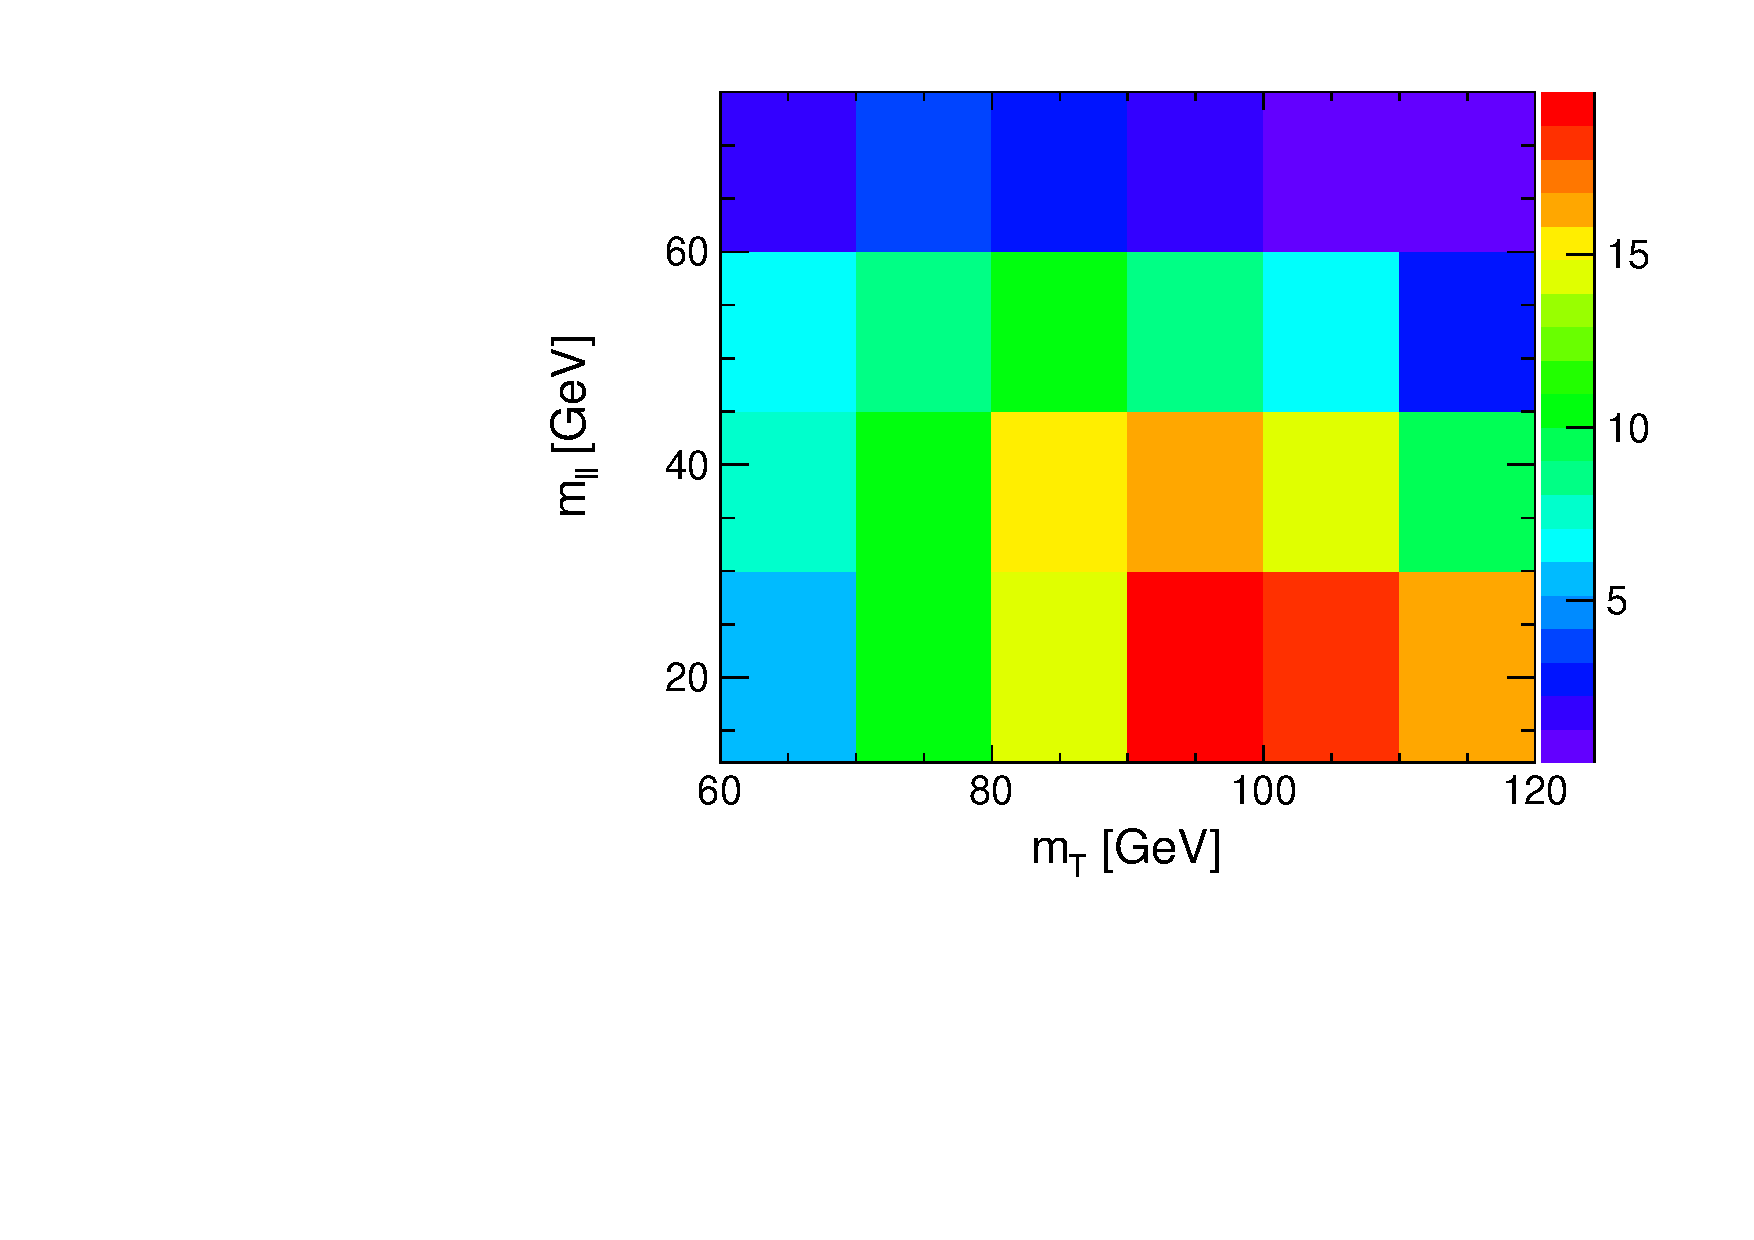
\includegraphics[width=.45\textwidth]{figures/mtvsmll_hww_0j.pdf}
}
\subfigure[Graviton ($2_m^+$), 0-Jet]{
\centering
\label{subfig:xww0j}
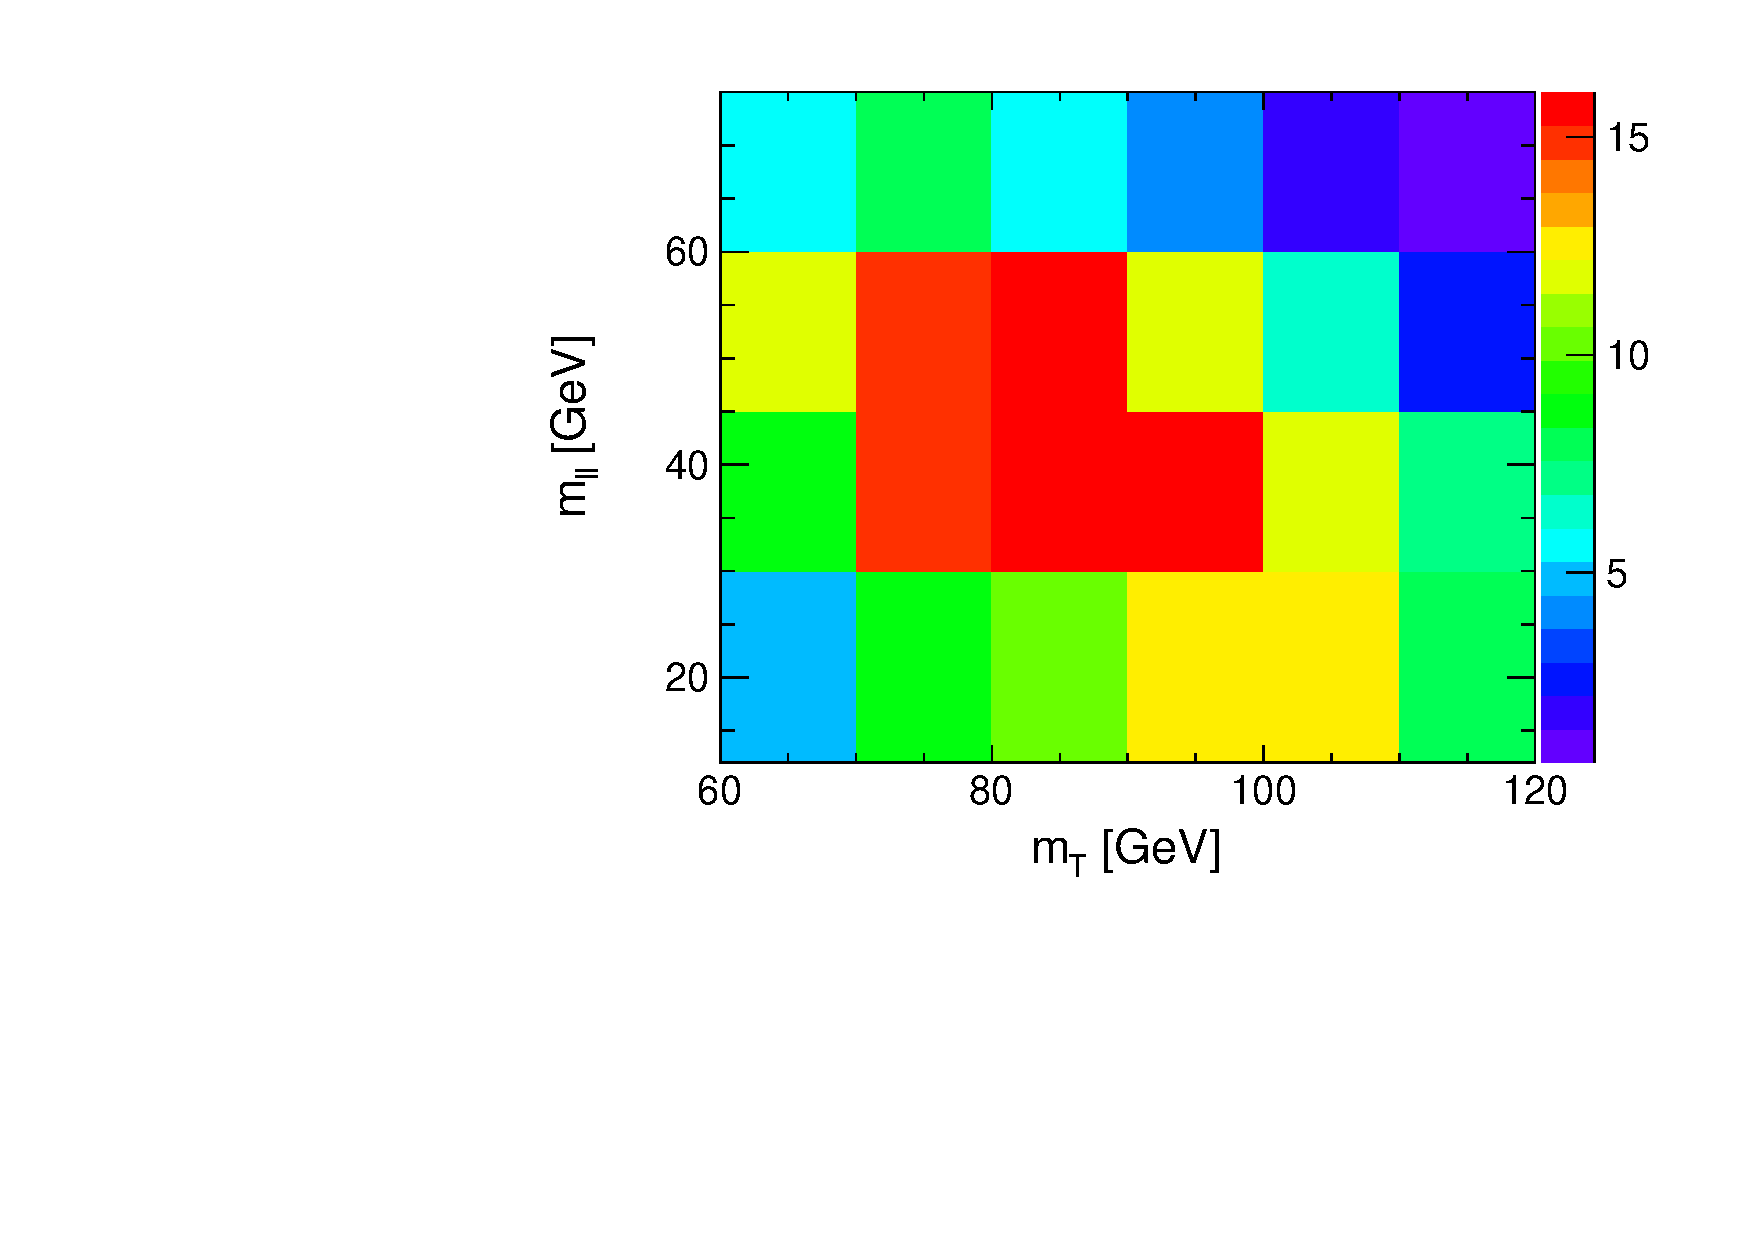
\includegraphics[width=.45\textwidth]{figures/mtvsmll_xww_0j.pdf}
}\\
\subfigure[SM Higgs, 1-Jet]{
\centering
\label{subfig:hww0j}
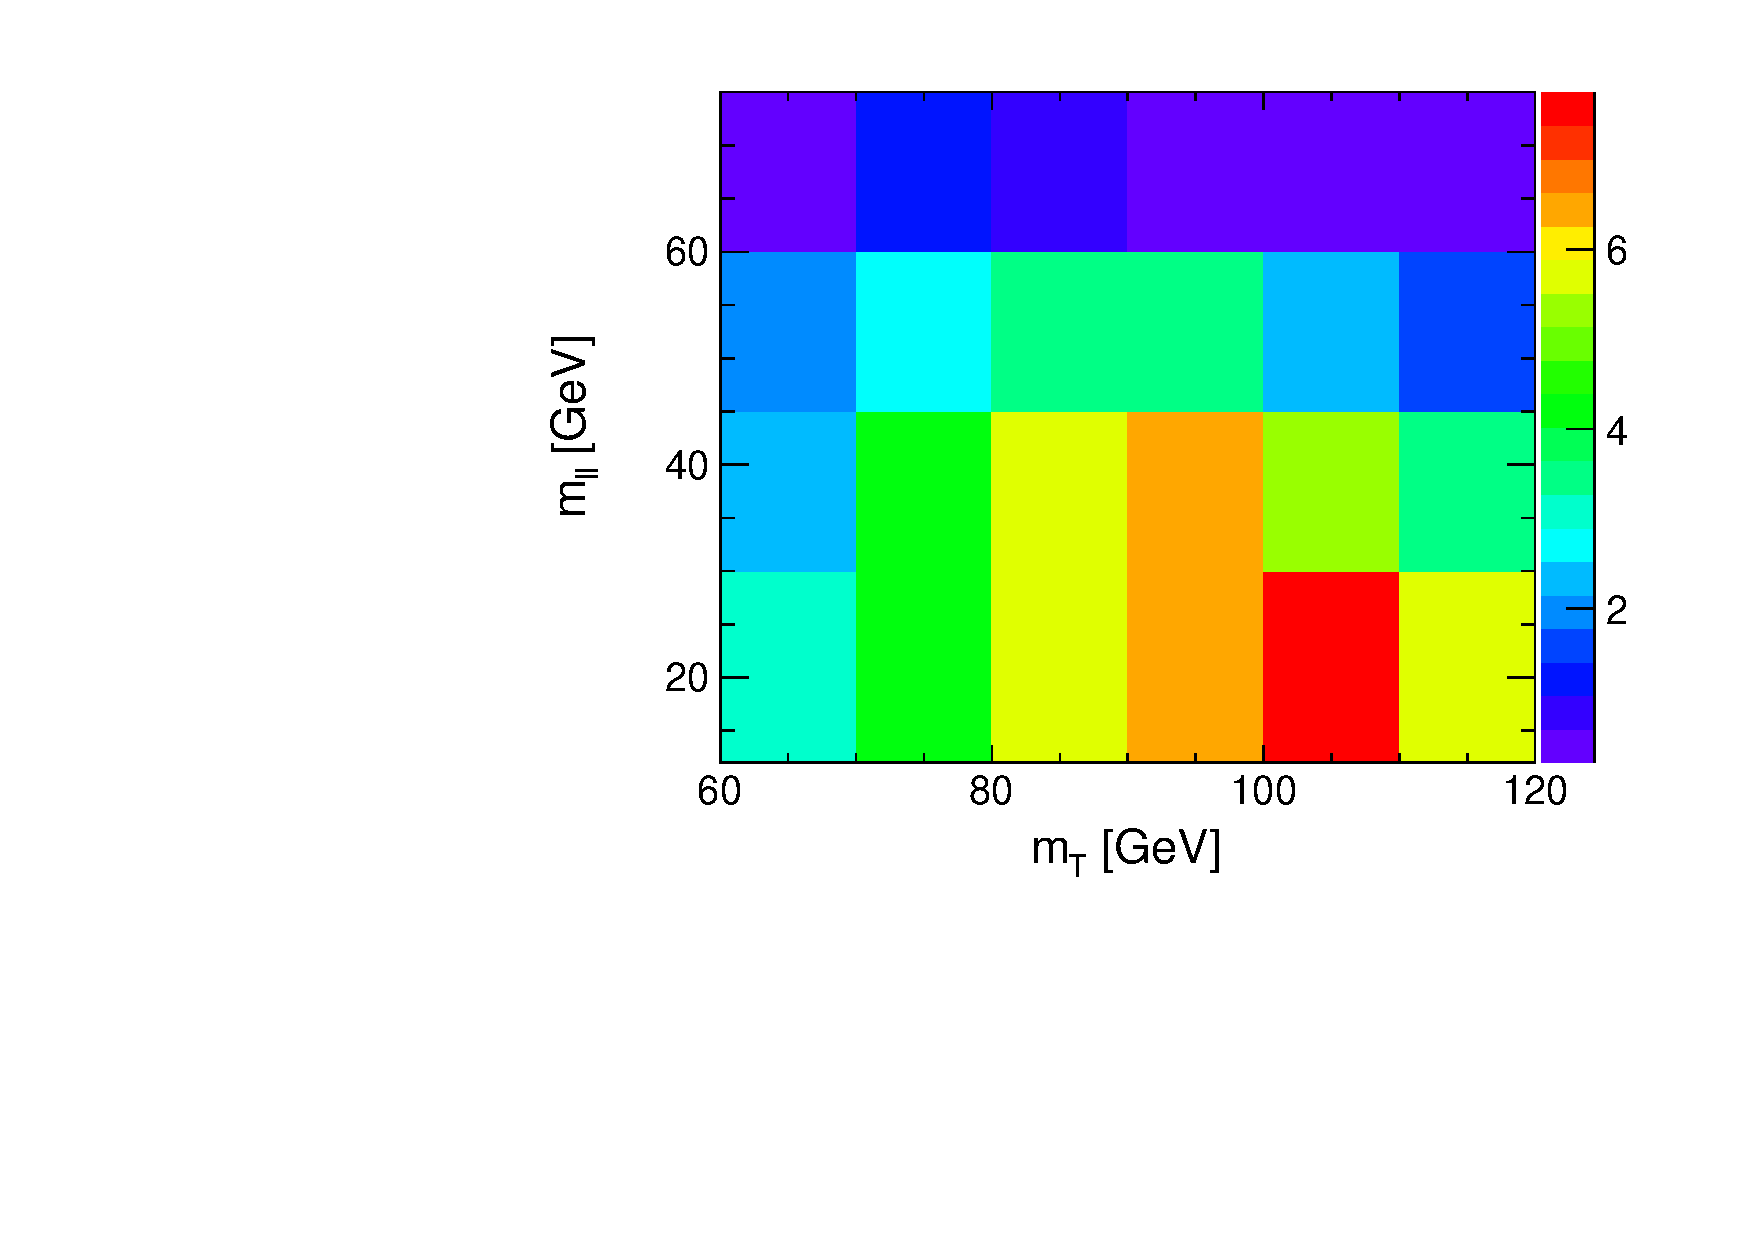
\includegraphics[width=.45\textwidth]{figures/mtvsmll_hww_1j.pdf}
}
\subfigure[Graviton ($2_m^+$), 1-Jet]{
\centering
\label{subfig:xww0j}
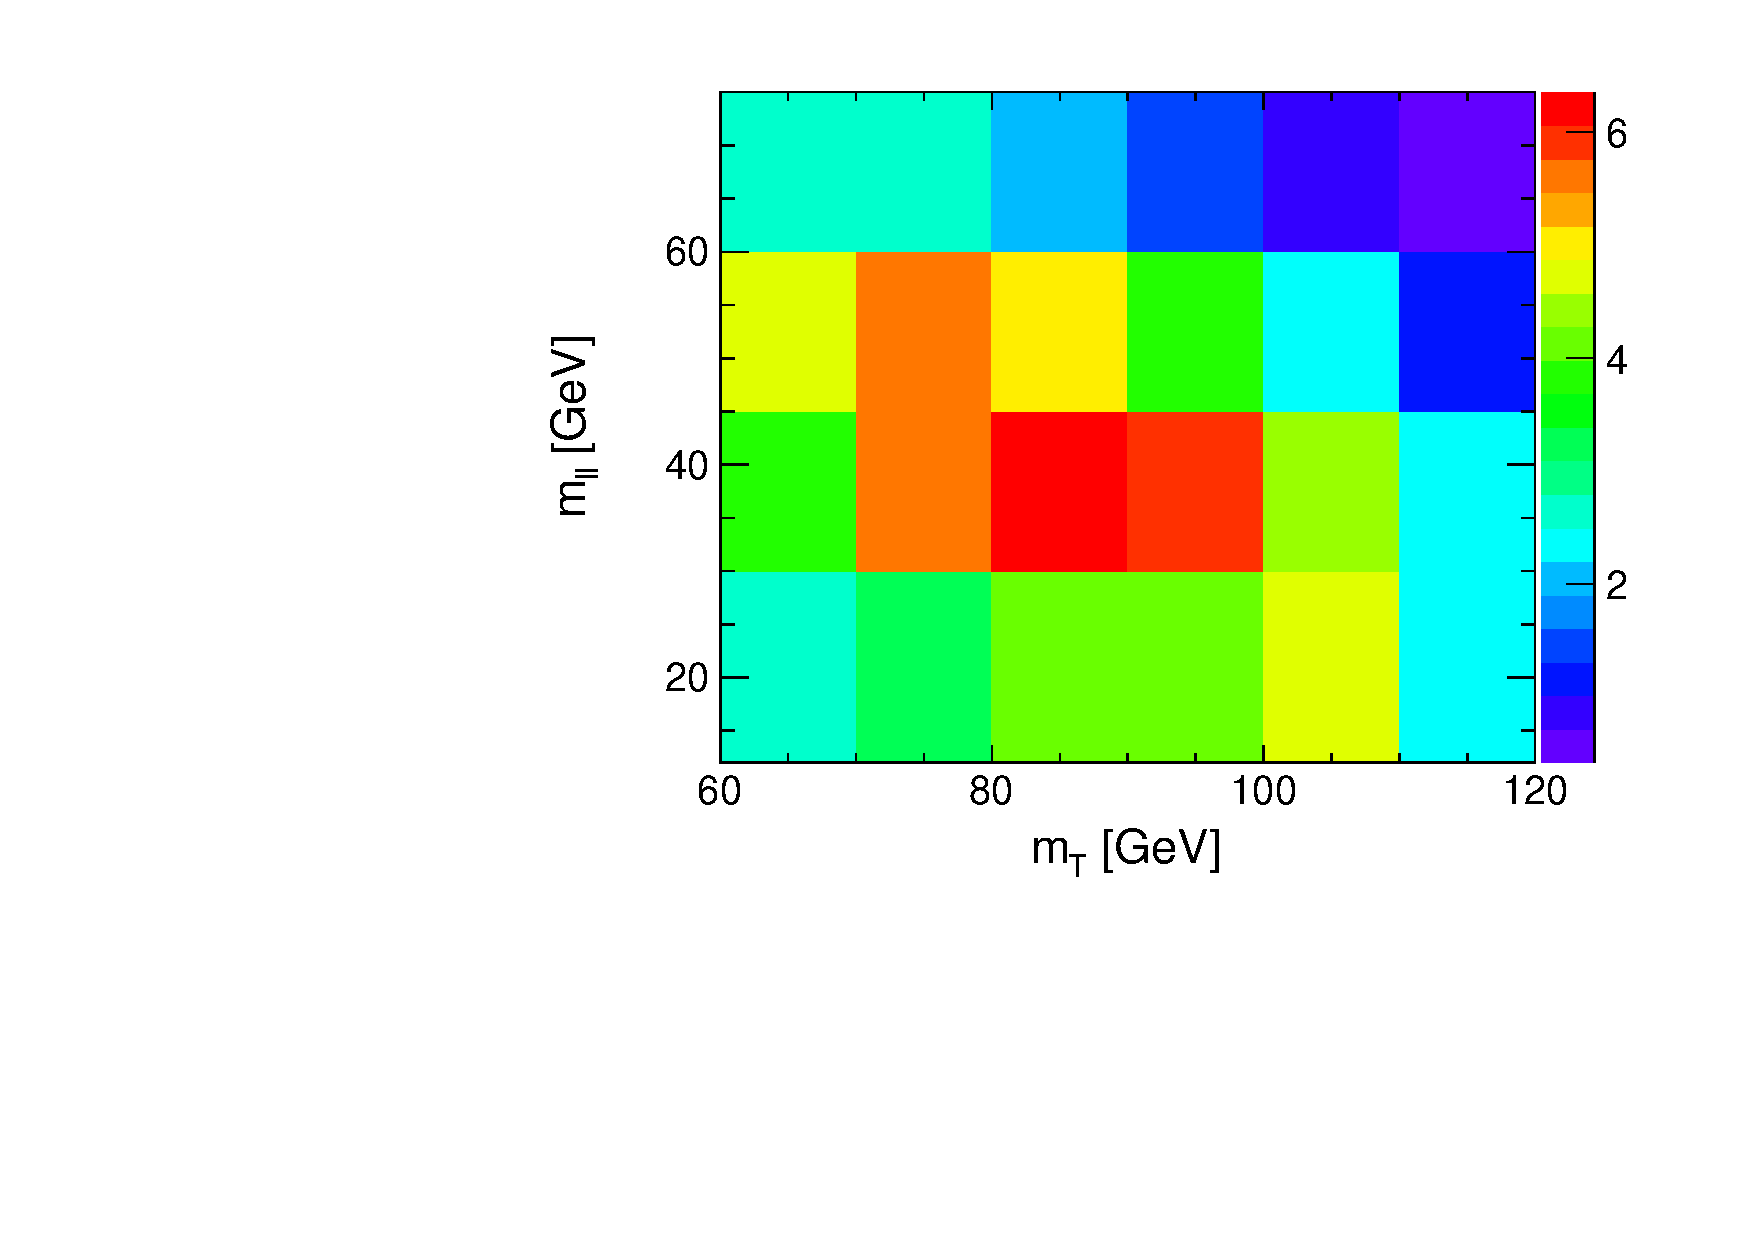
\includegraphics[width=.45\textwidth]{figures/mtvsmll_xww_1j.pdf}
}\\
\caption{The $m_T-m_{\ell\ell}$ templates for the SM Higgs and 
spin 2 graviton like resonances, zoomed in 
the signal regions. The distributions are 
normalized to the expectations for \intlumiEightTeV.}
\label{fig:mtvsmll_sig}
\end{figure}
%%%%%%%%%%%%%%%%%%%%%%%%%%%%%%%%%%%%%%%%%%%%%


%%%%%%%%%%%%%%%%%%%%%%%%%%%%%%%%%%%%%%%%%%%%%
\begin{figure}[!hbtp]
\centering
\subfigure[$qq\to WW$]{
\centering
\label{subfig:qqww}
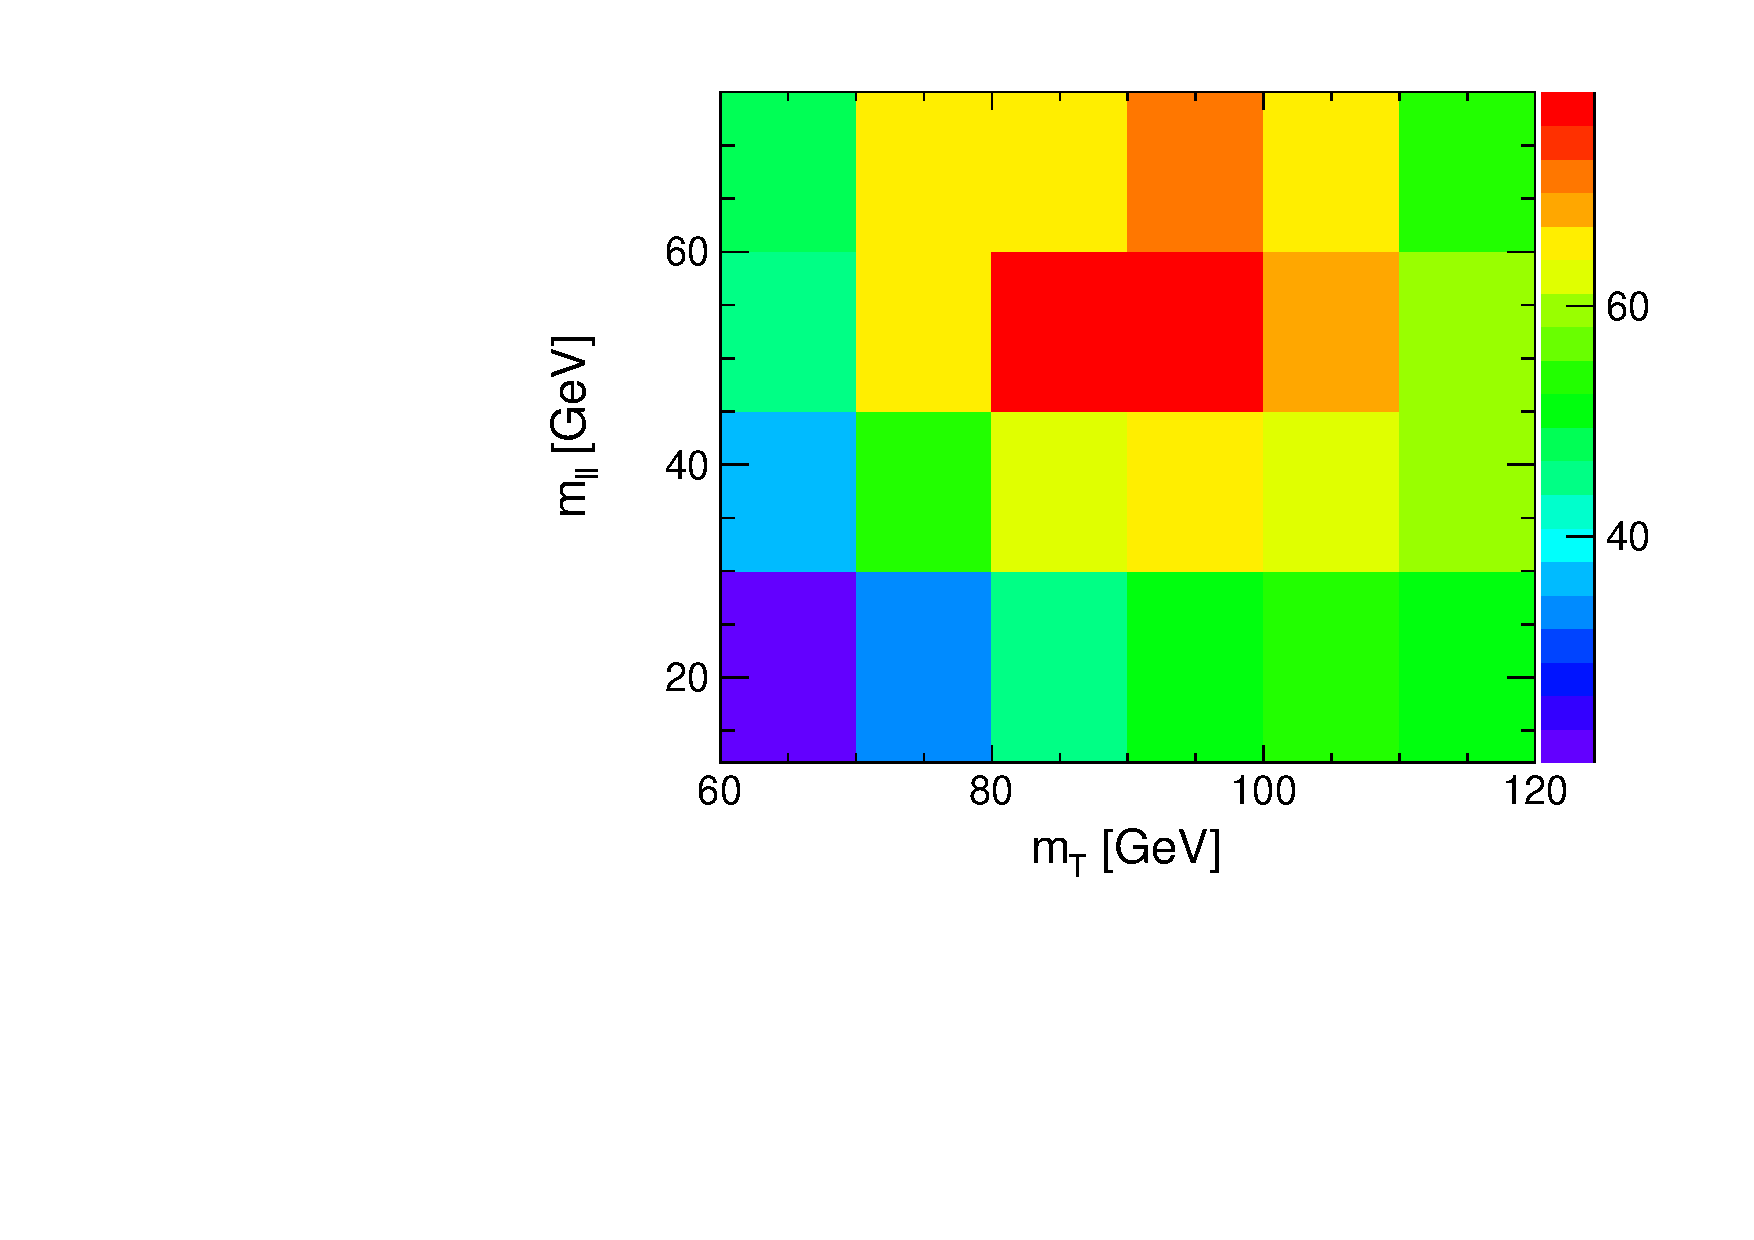
\includegraphics[width=.45\textwidth]{figures/mtvsmll_qqWW_0j.pdf}
}
\subfigure[Top]{
\centering
\label{subfig:top}
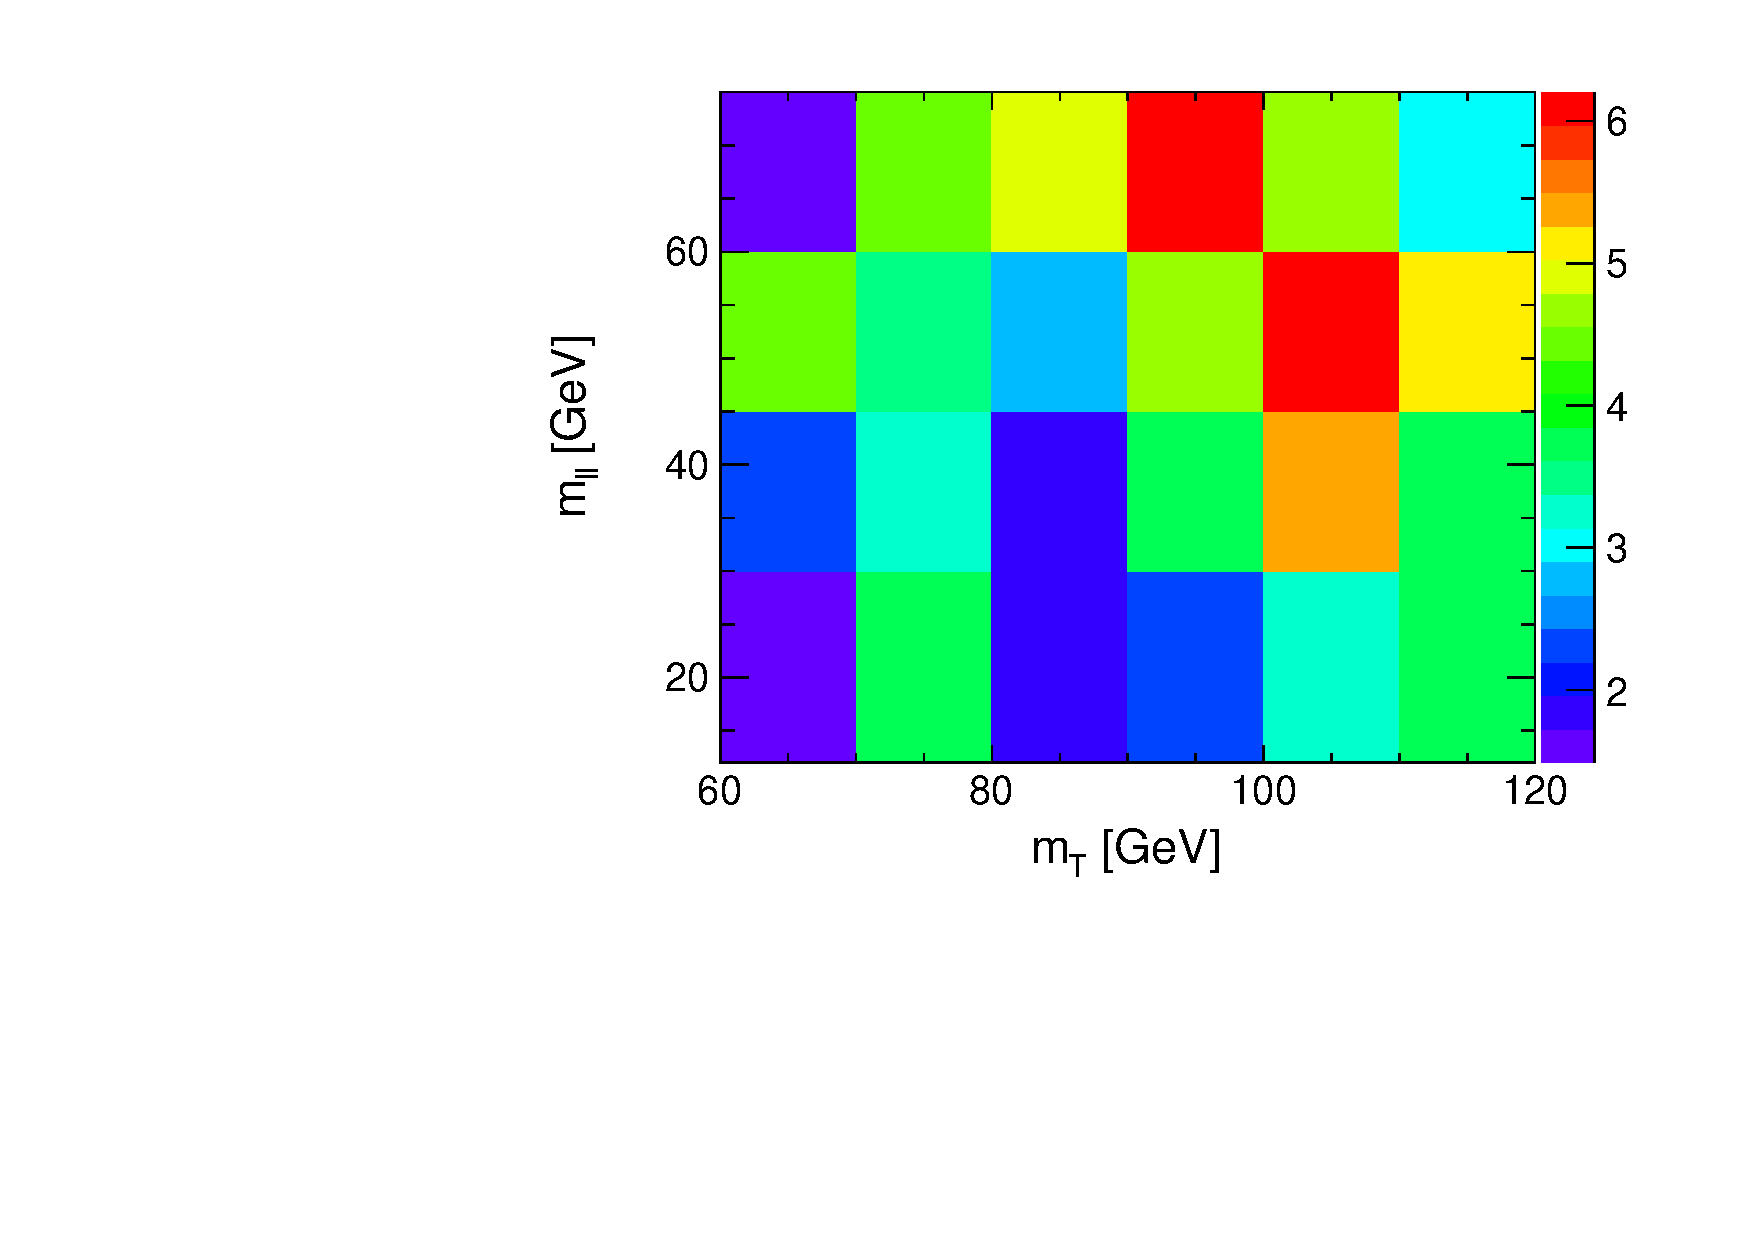
\includegraphics[width=.45\textwidth]{figures/mtvsmll_Top_0j.pdf}
}\\
\subfigure[W+Jets(E)]{
\centering
\label{subfig:wjetse}
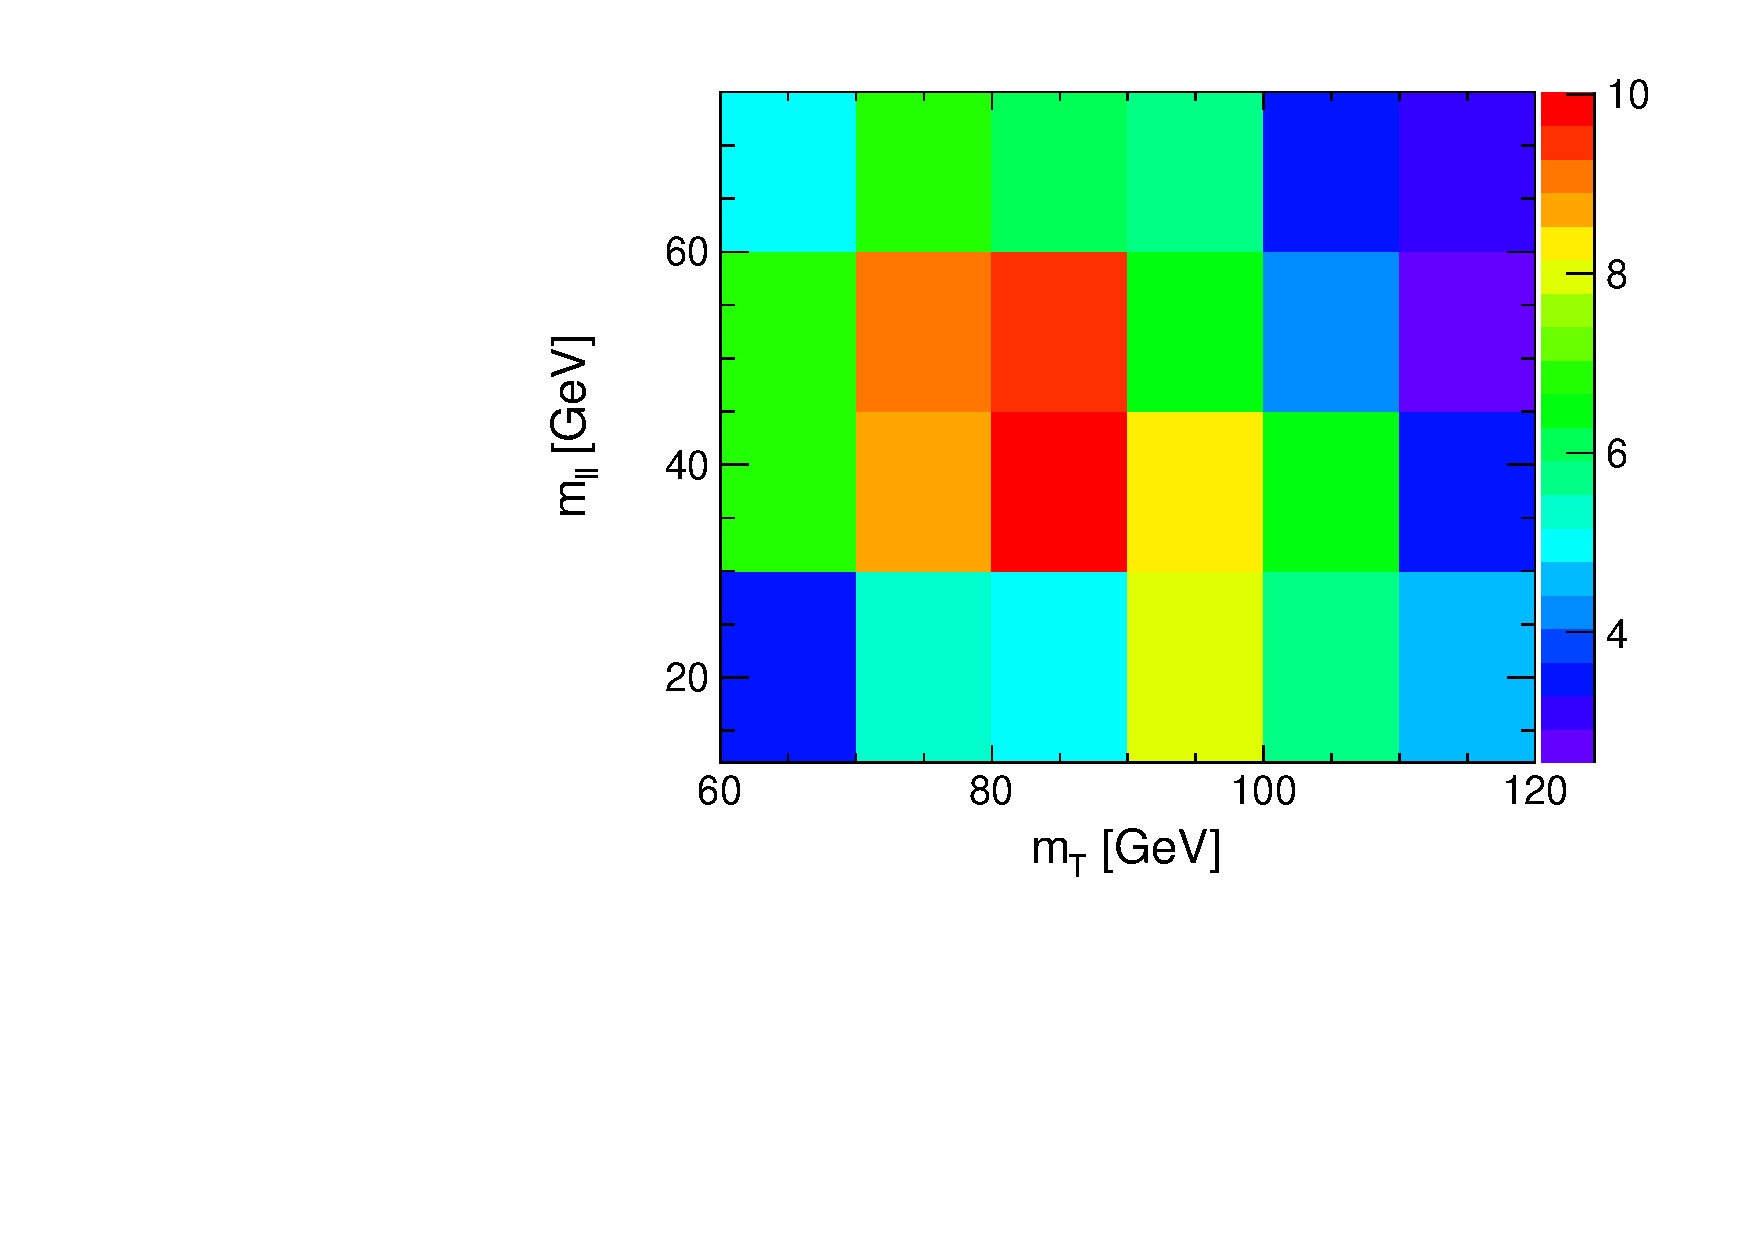
\includegraphics[width=.45\textwidth]{figures/mtvsmll_WjetsE_0j.pdf}
}
\subfigure[W+Jets(M)]{
\centering
\label{subfig:wjetse}
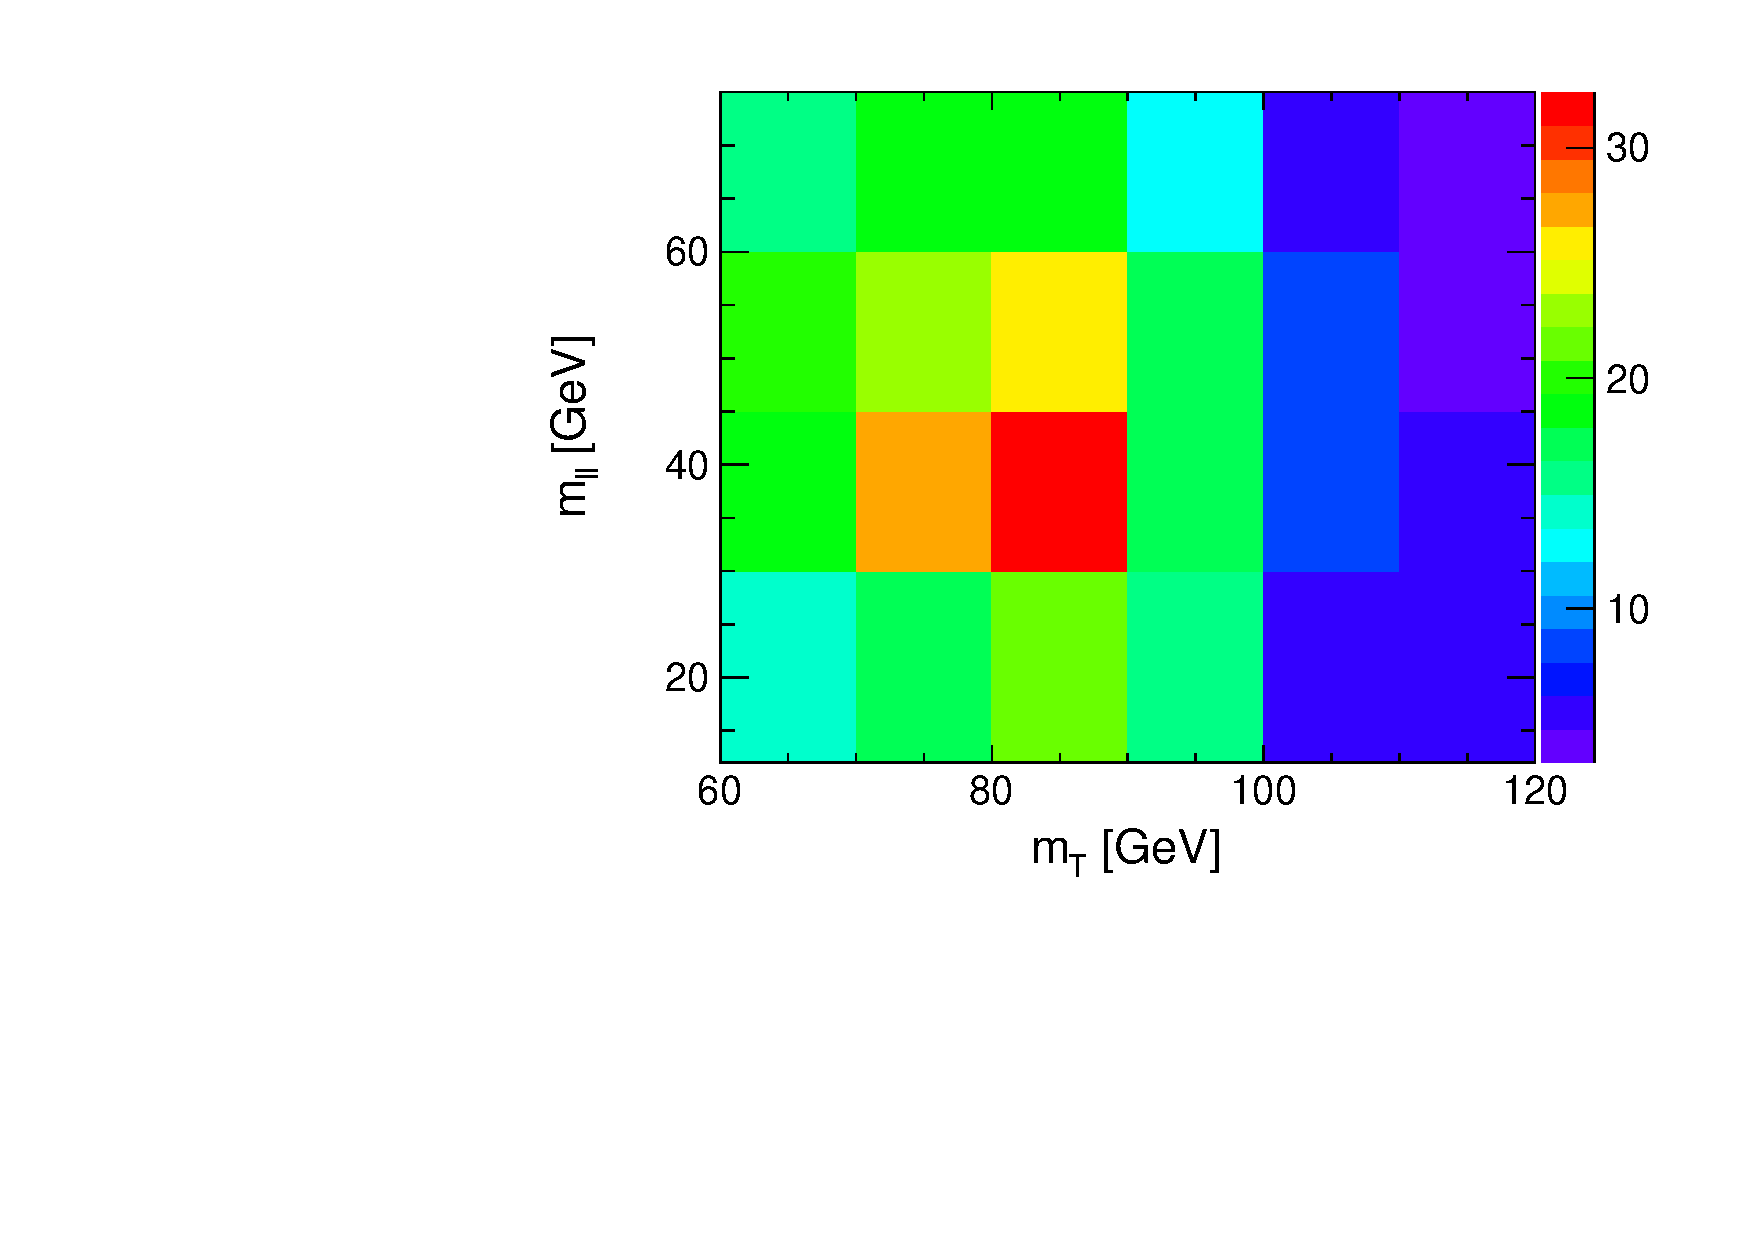
\includegraphics[width=.45\textwidth]{figures/mtvsmll_WjetsM_0j.pdf}
}\\
\subfigure[$W\gamma$]{
\centering
\label{subfig:wgamma}
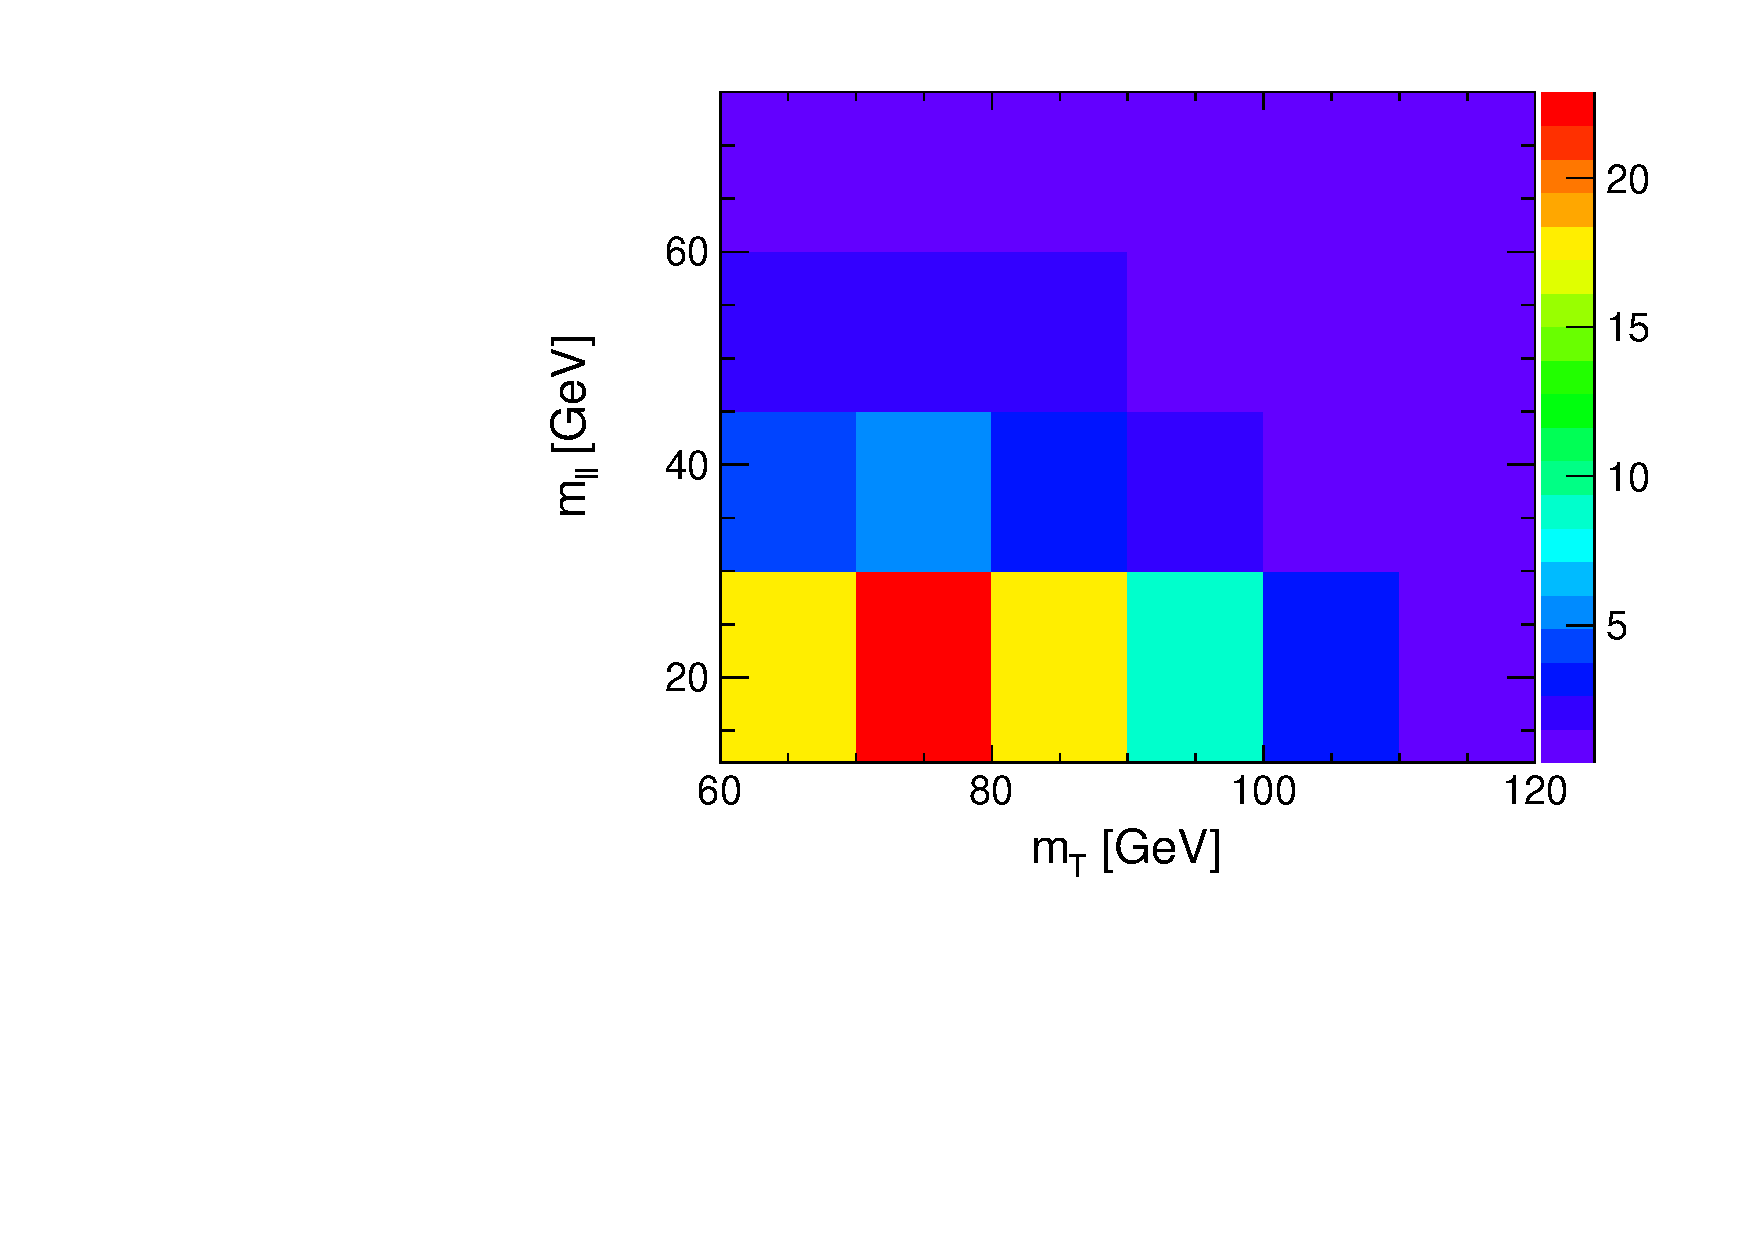
\includegraphics[width=.45\textwidth]{figures/mtvsmll_Wgamma_0j.pdf}
}
\subfigure[$W\gamma^*$]{
\centering
\label{subfig:wgst}
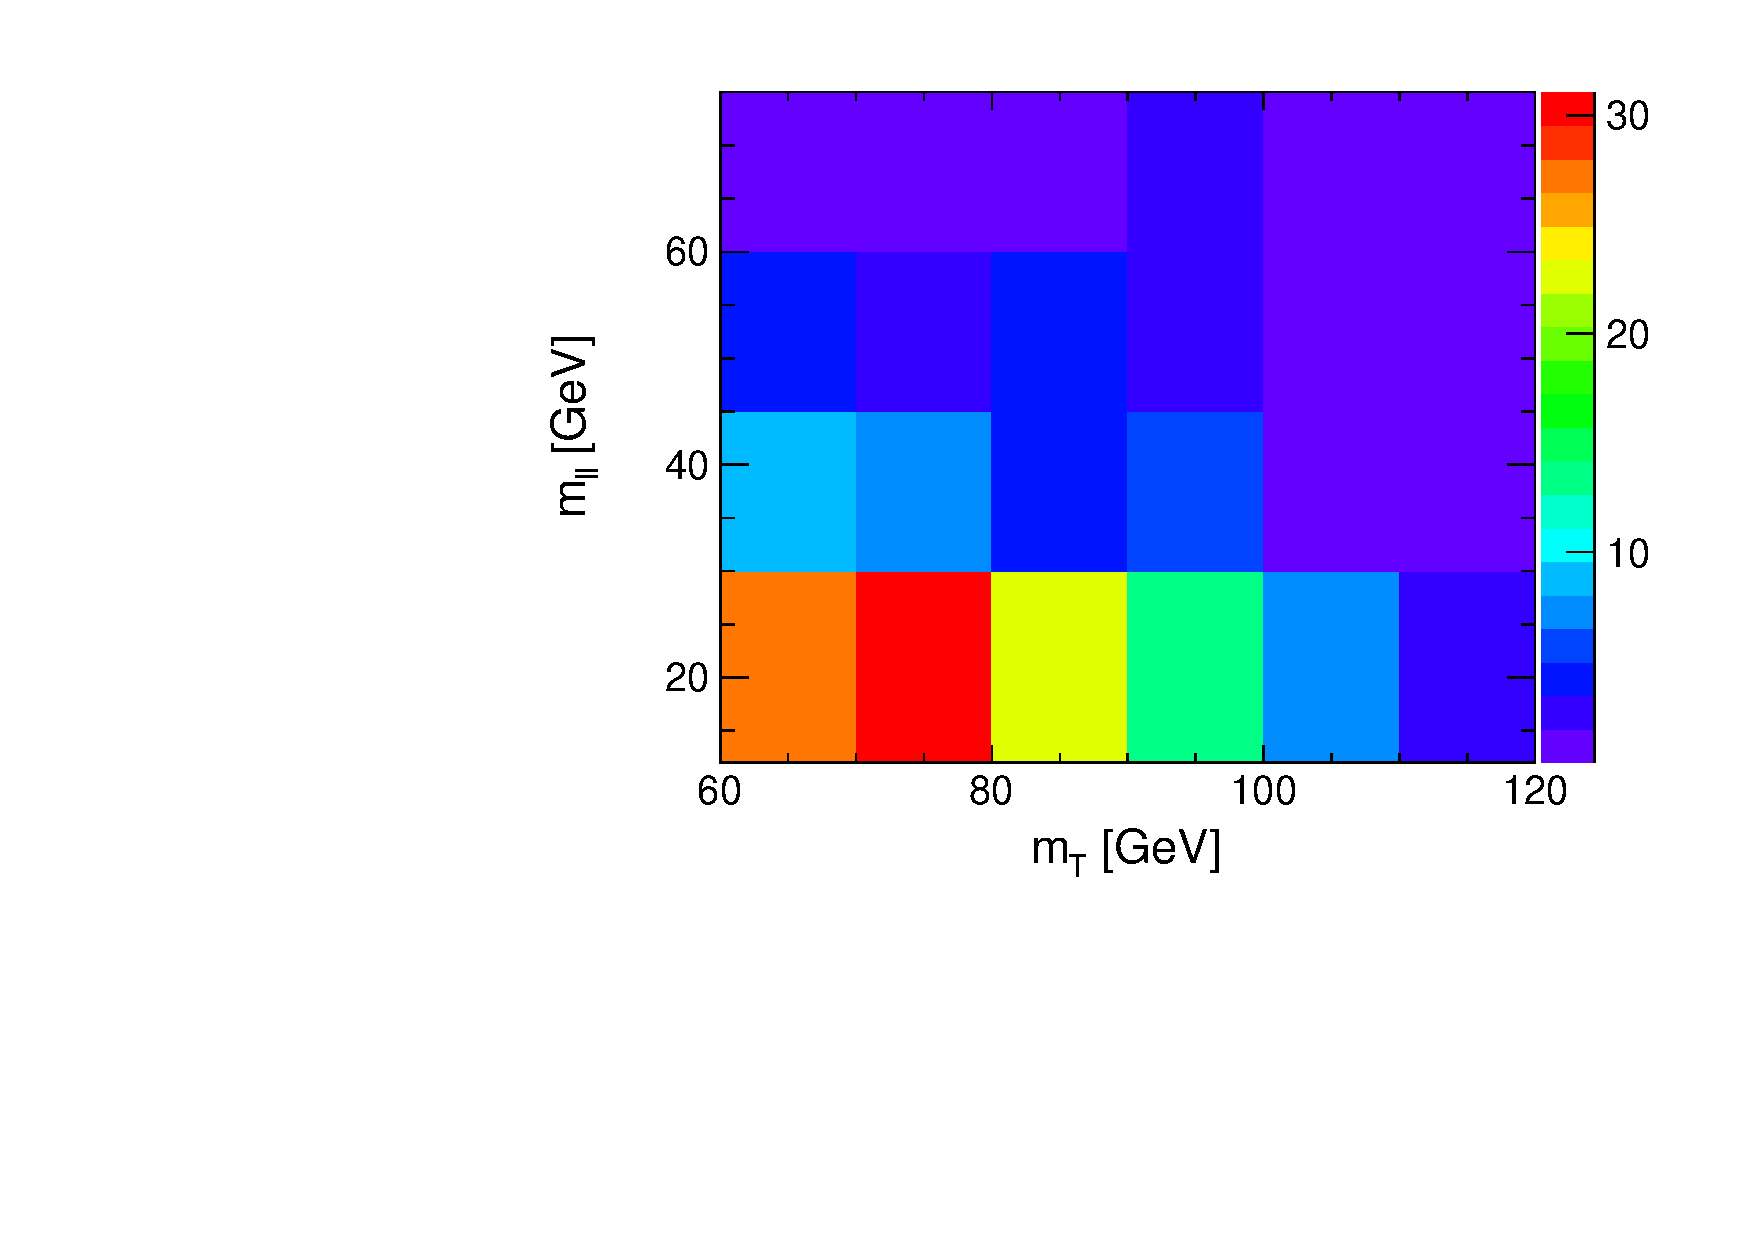
\includegraphics[width=.45\textwidth]{figures/mtvsmll_Wgstar_0j.pdf}
}\\
\caption{The $m_T-m_{\ell\ell}$ templates for the backgrounds, zoomed in 
the signal regions in the {\bf 0-Jet} bin. The distributions are 
normalized to the expectations for \intlumiEightTeV.}
\label{fig:mtvsmll_bkg_0j}
\end{figure}
%%%%%%%%%%%%%%%%%%%%%%%%%%%%%%%%%%%%%%%%%%%%%

%%%%%%%%%%%%%%%%%%%%%%%%%%%%%%%%%%%%%%%%%%%%%
\begin{figure}[!hbtp]
\centering
\subfigure[$qq\to WW$]{
\centering
\label{subfig:qqww}
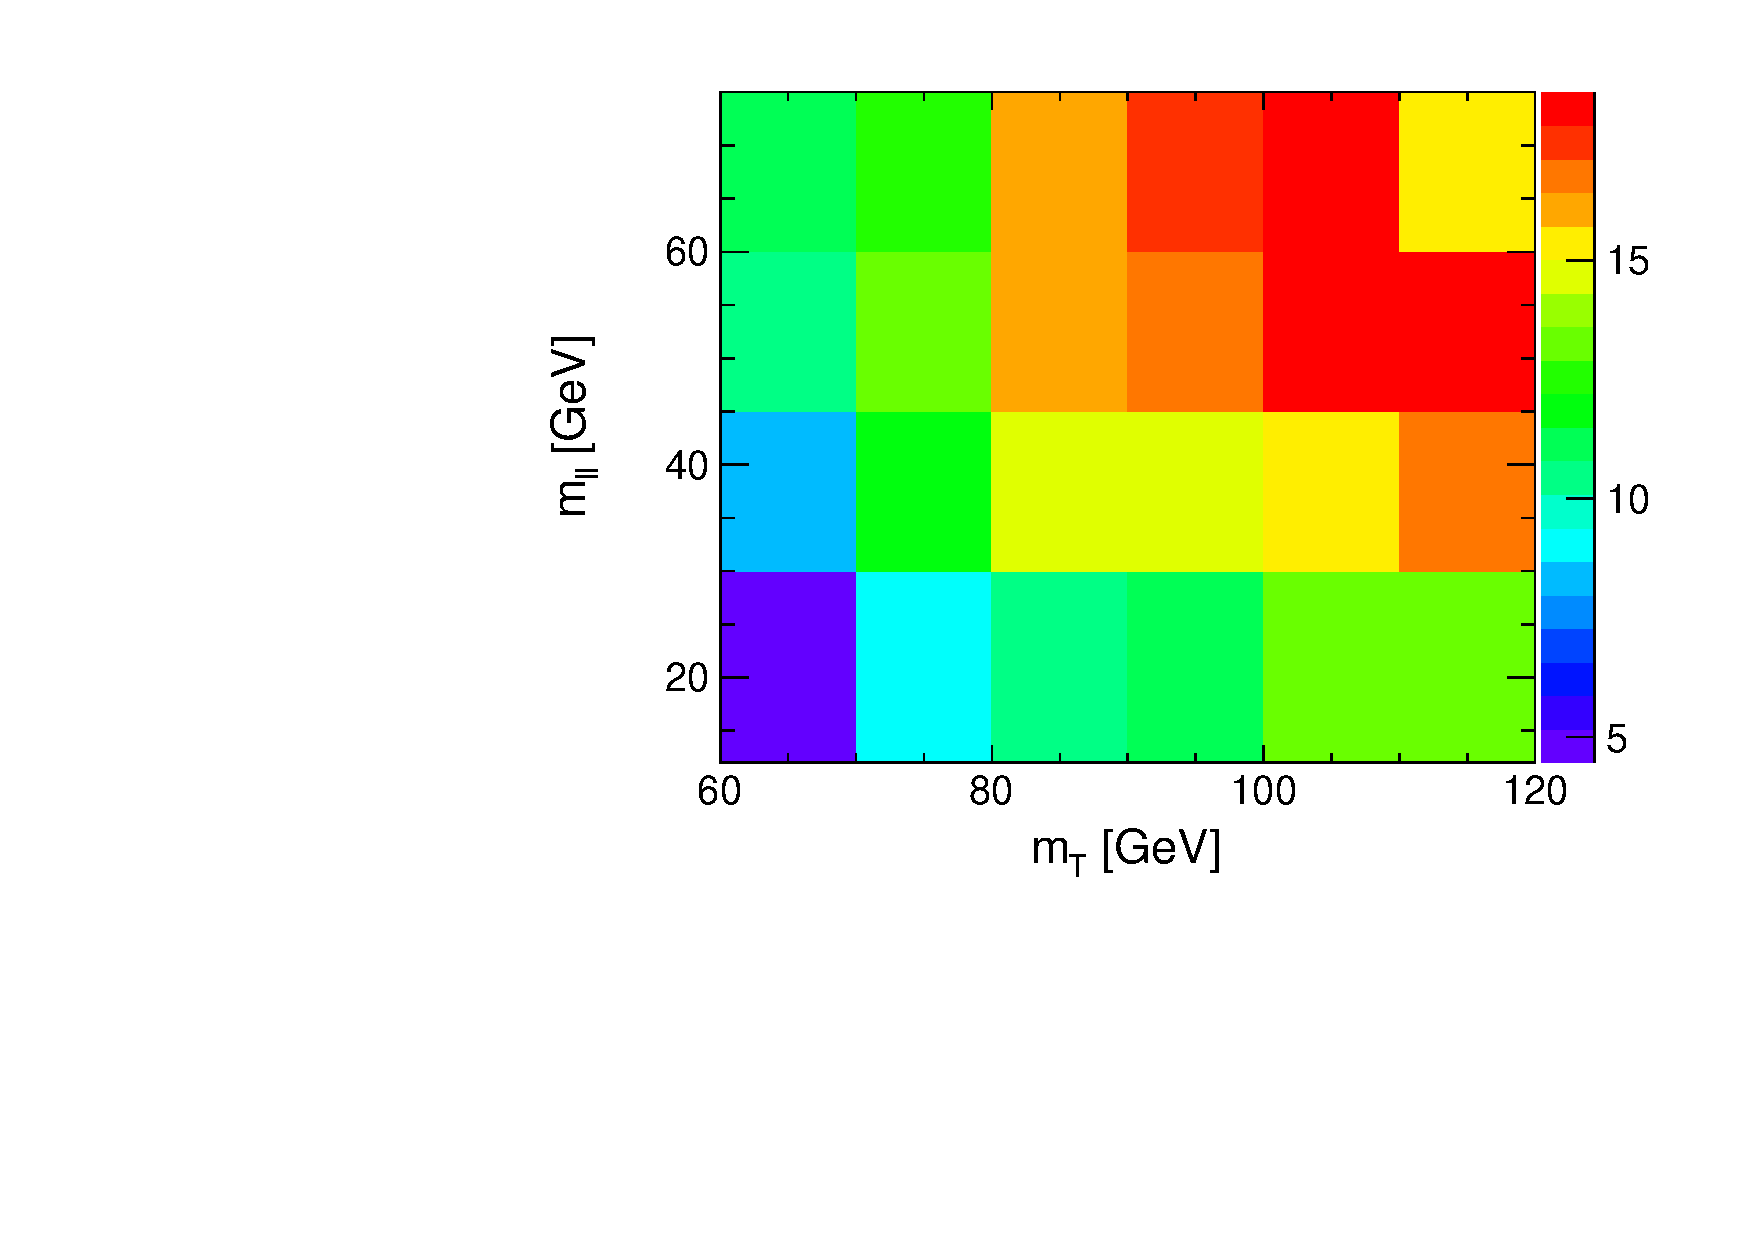
\includegraphics[width=.45\textwidth]{figures/mtvsmll_qqWW_1j.pdf}
}
\subfigure[Top]{
\centering
\label{subfig:top}
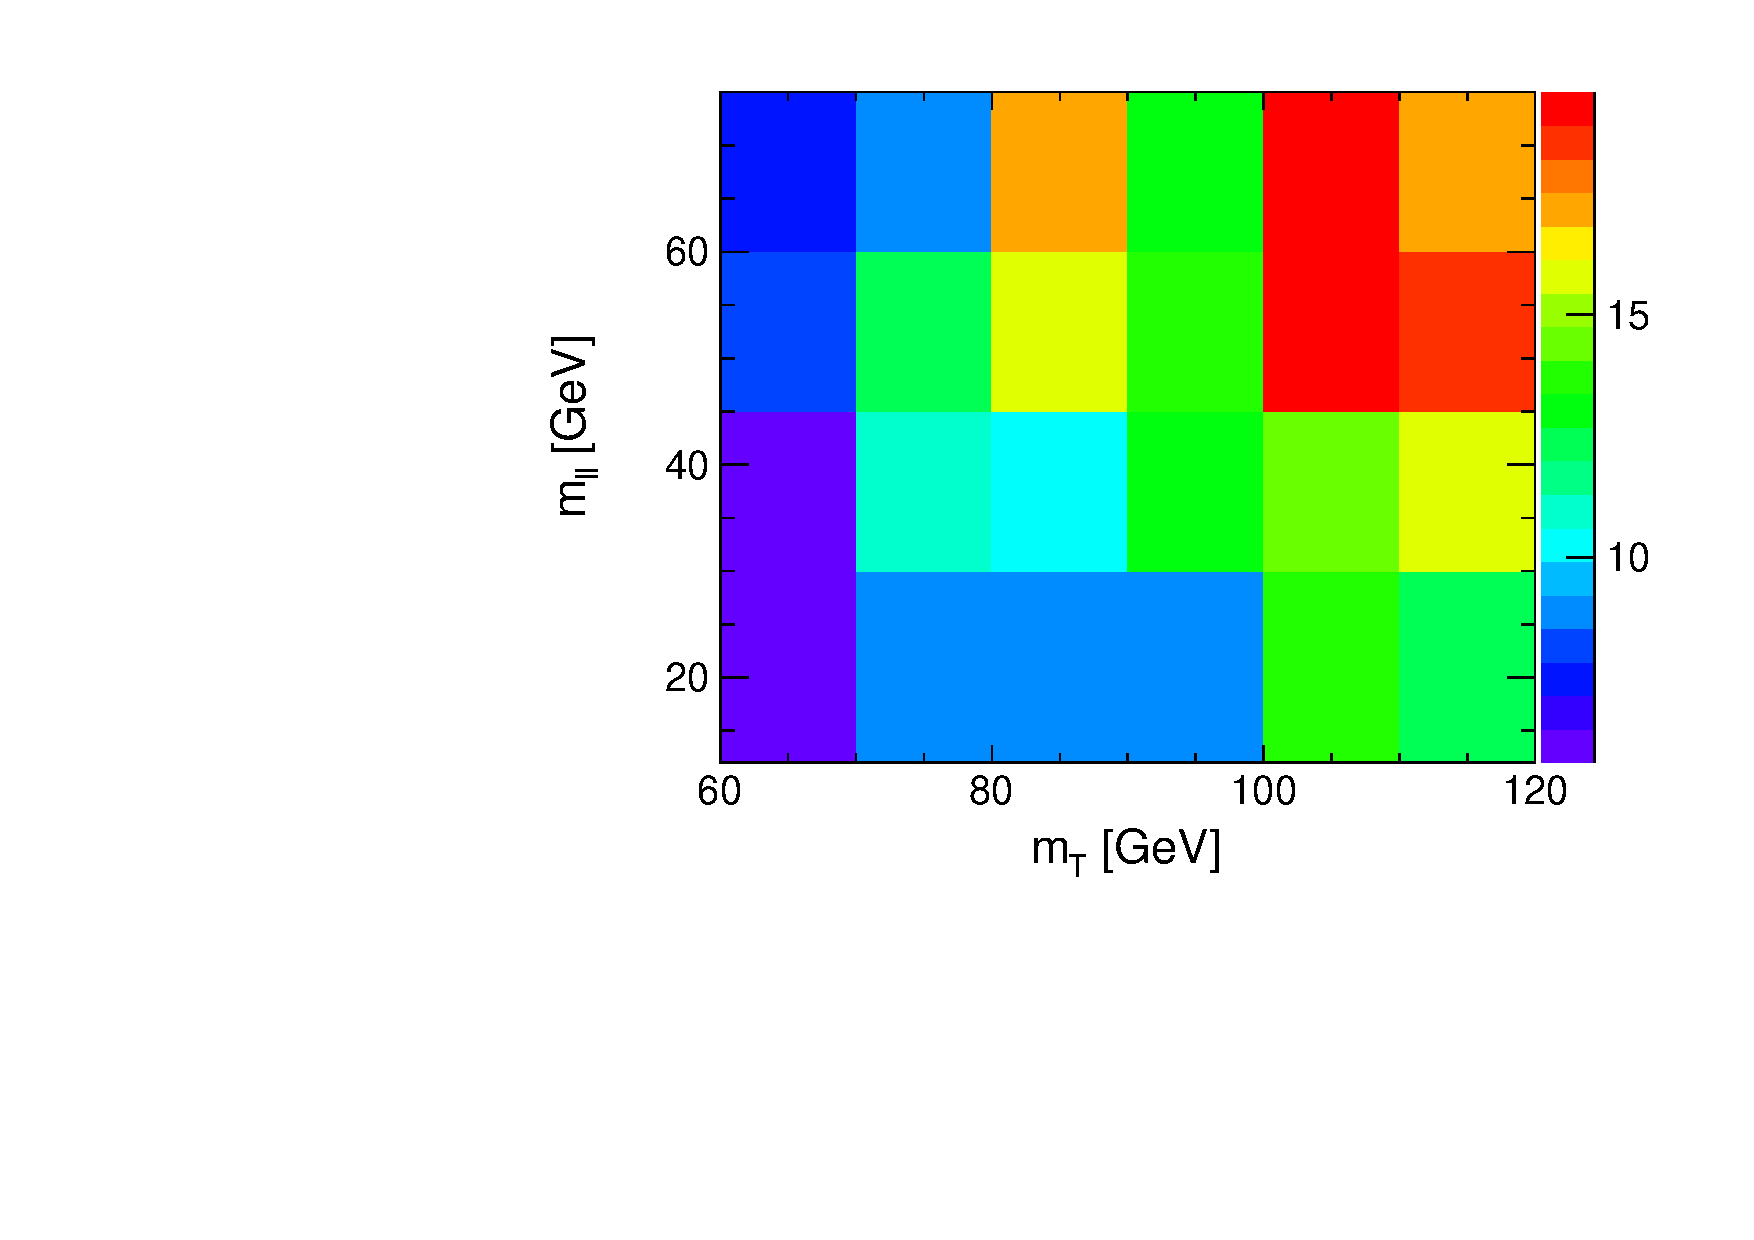
\includegraphics[width=.45\textwidth]{figures/mtvsmll_Top_1j.pdf}
}\\
\subfigure[W+Jets(E)]{
\centering
\label{subfig:wjetse}
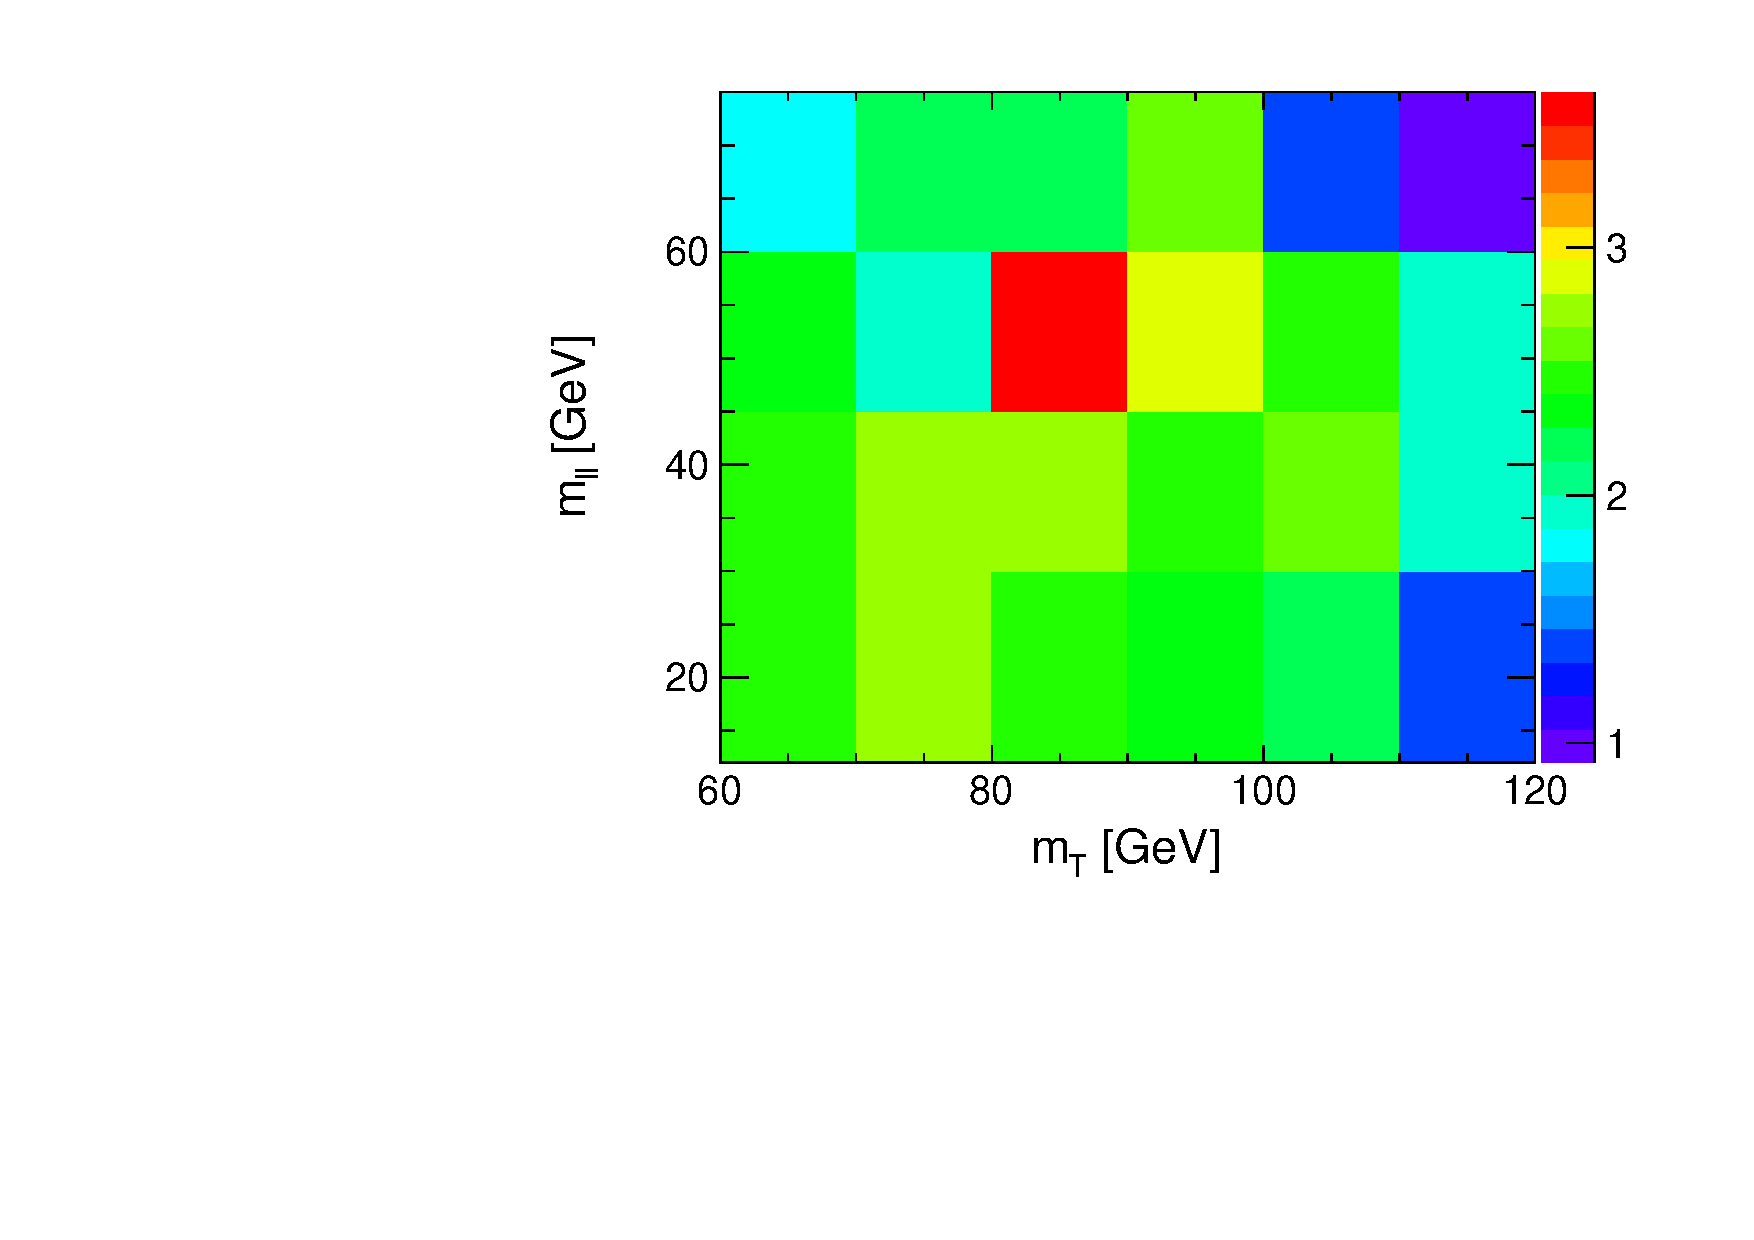
\includegraphics[width=.45\textwidth]{figures/mtvsmll_WjetsE_1j.pdf}
}
\subfigure[W+Jets(M)]{
\centering
\label{subfig:wjetse}
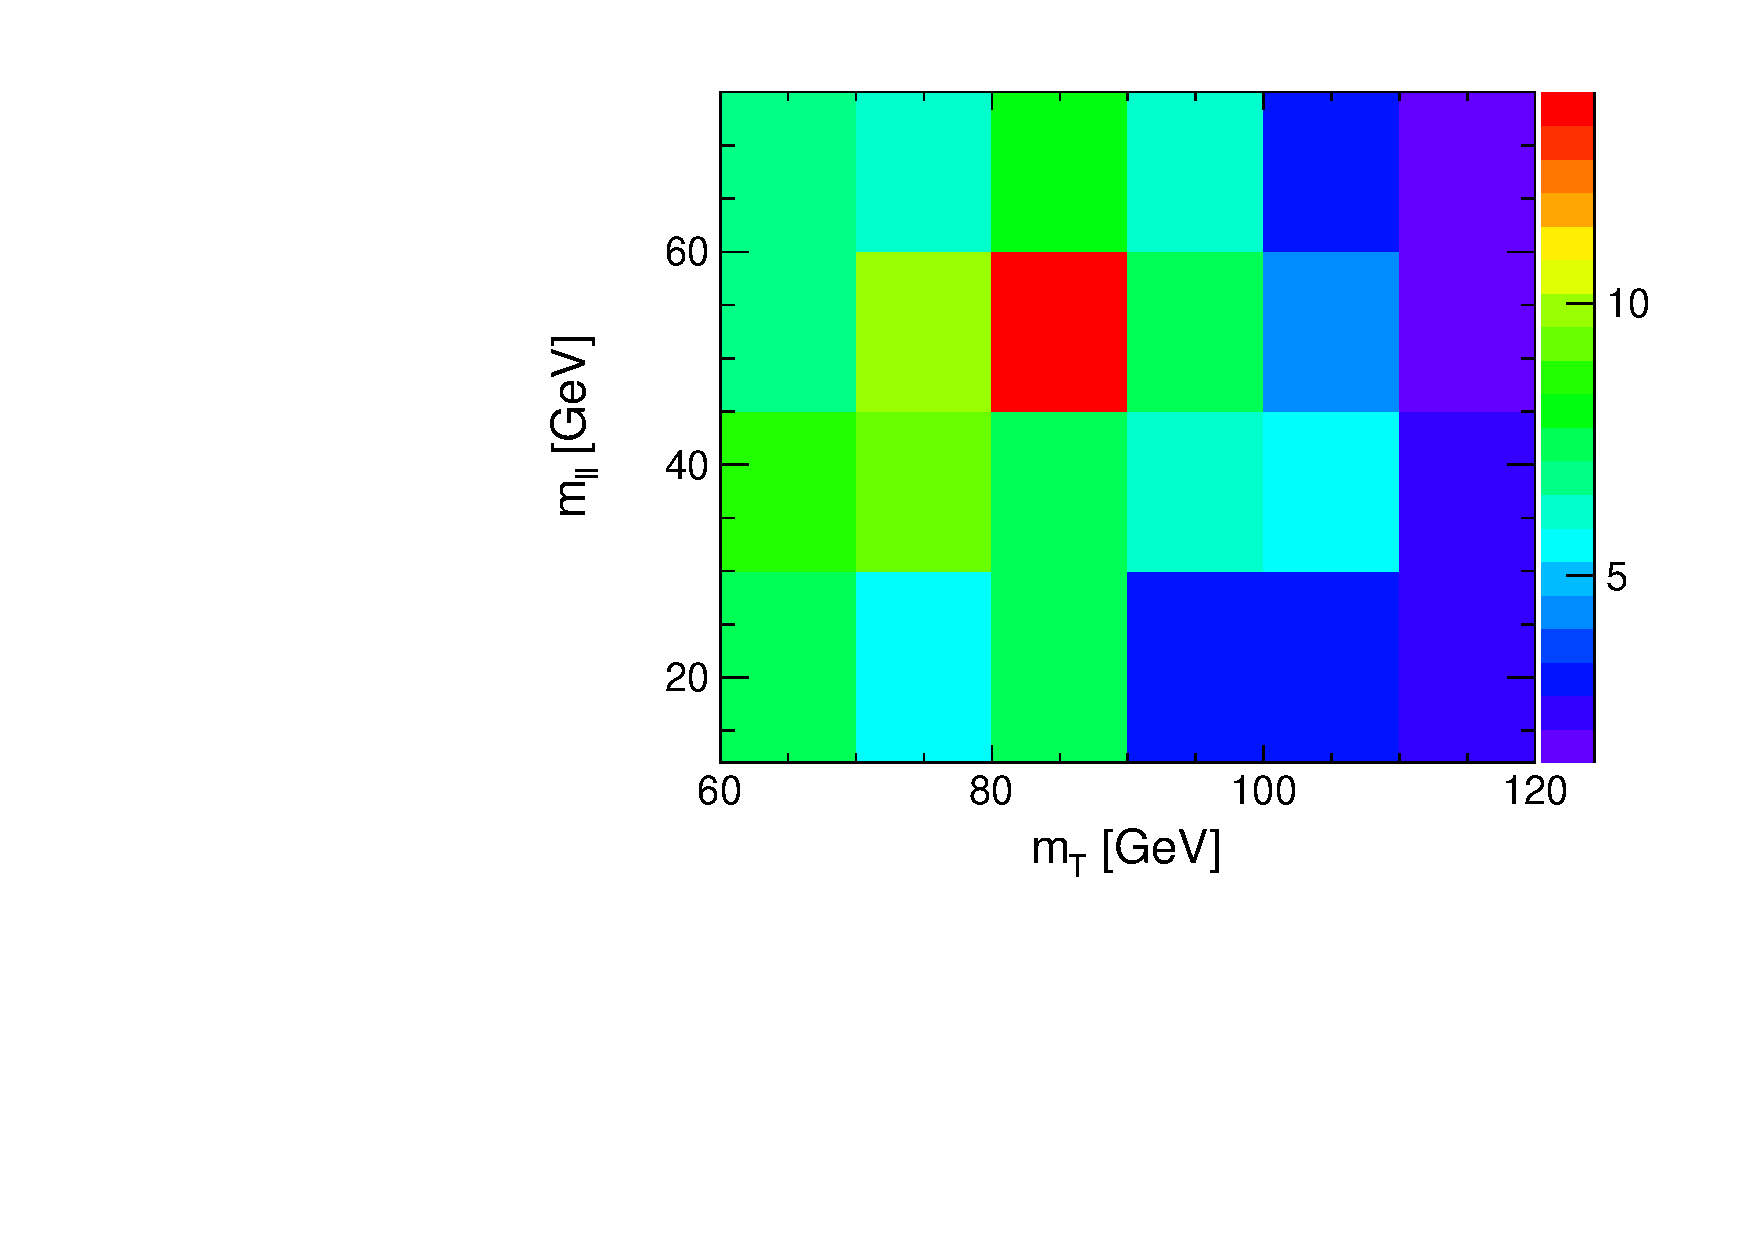
\includegraphics[width=.45\textwidth]{figures/mtvsmll_WjetsM_1j.pdf}
}\\
\subfigure[$W\gamma$]{
\centering
\label{subfig:wgamma}
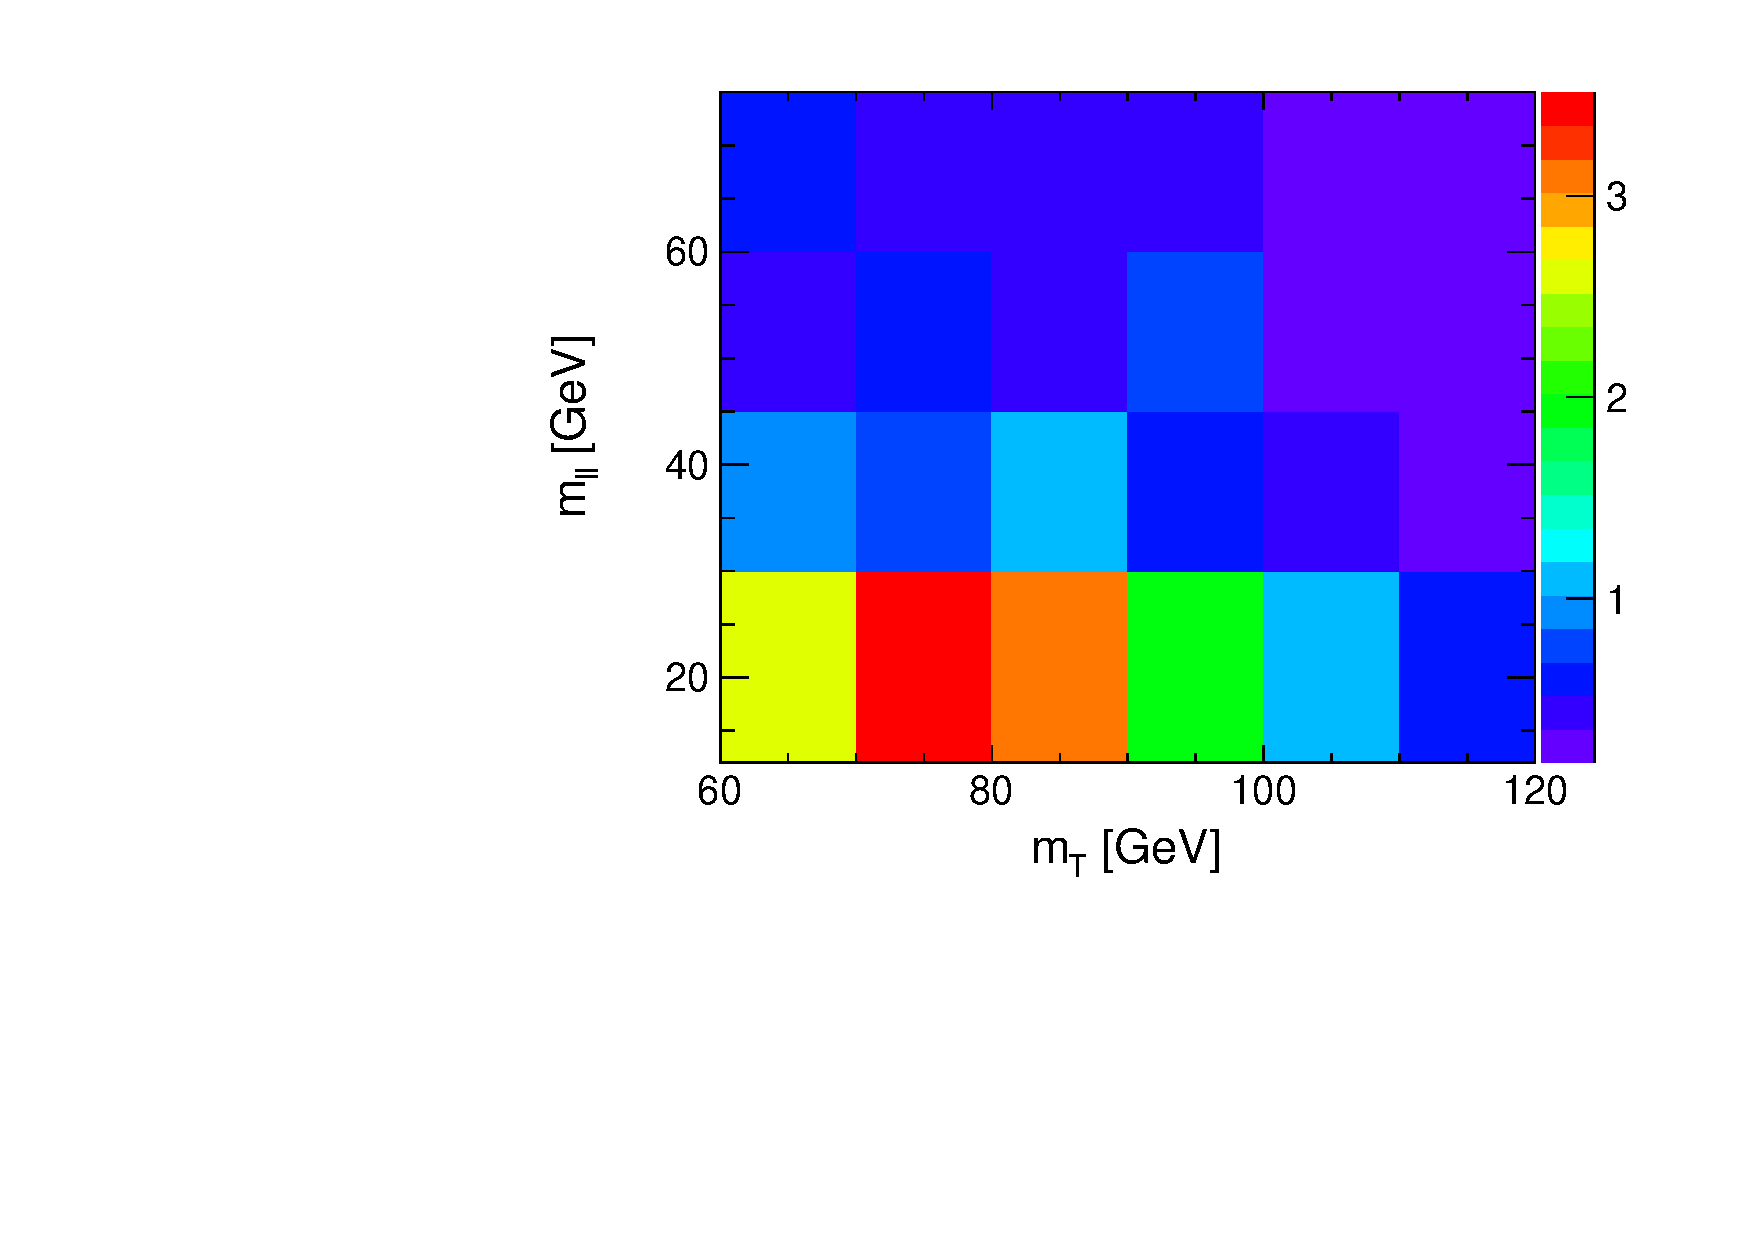
\includegraphics[width=.45\textwidth]{figures/mtvsmll_Wgamma_1j.pdf}
}
\subfigure[$W\gamma^*$]{
\centering
\label{subfig:wgst}
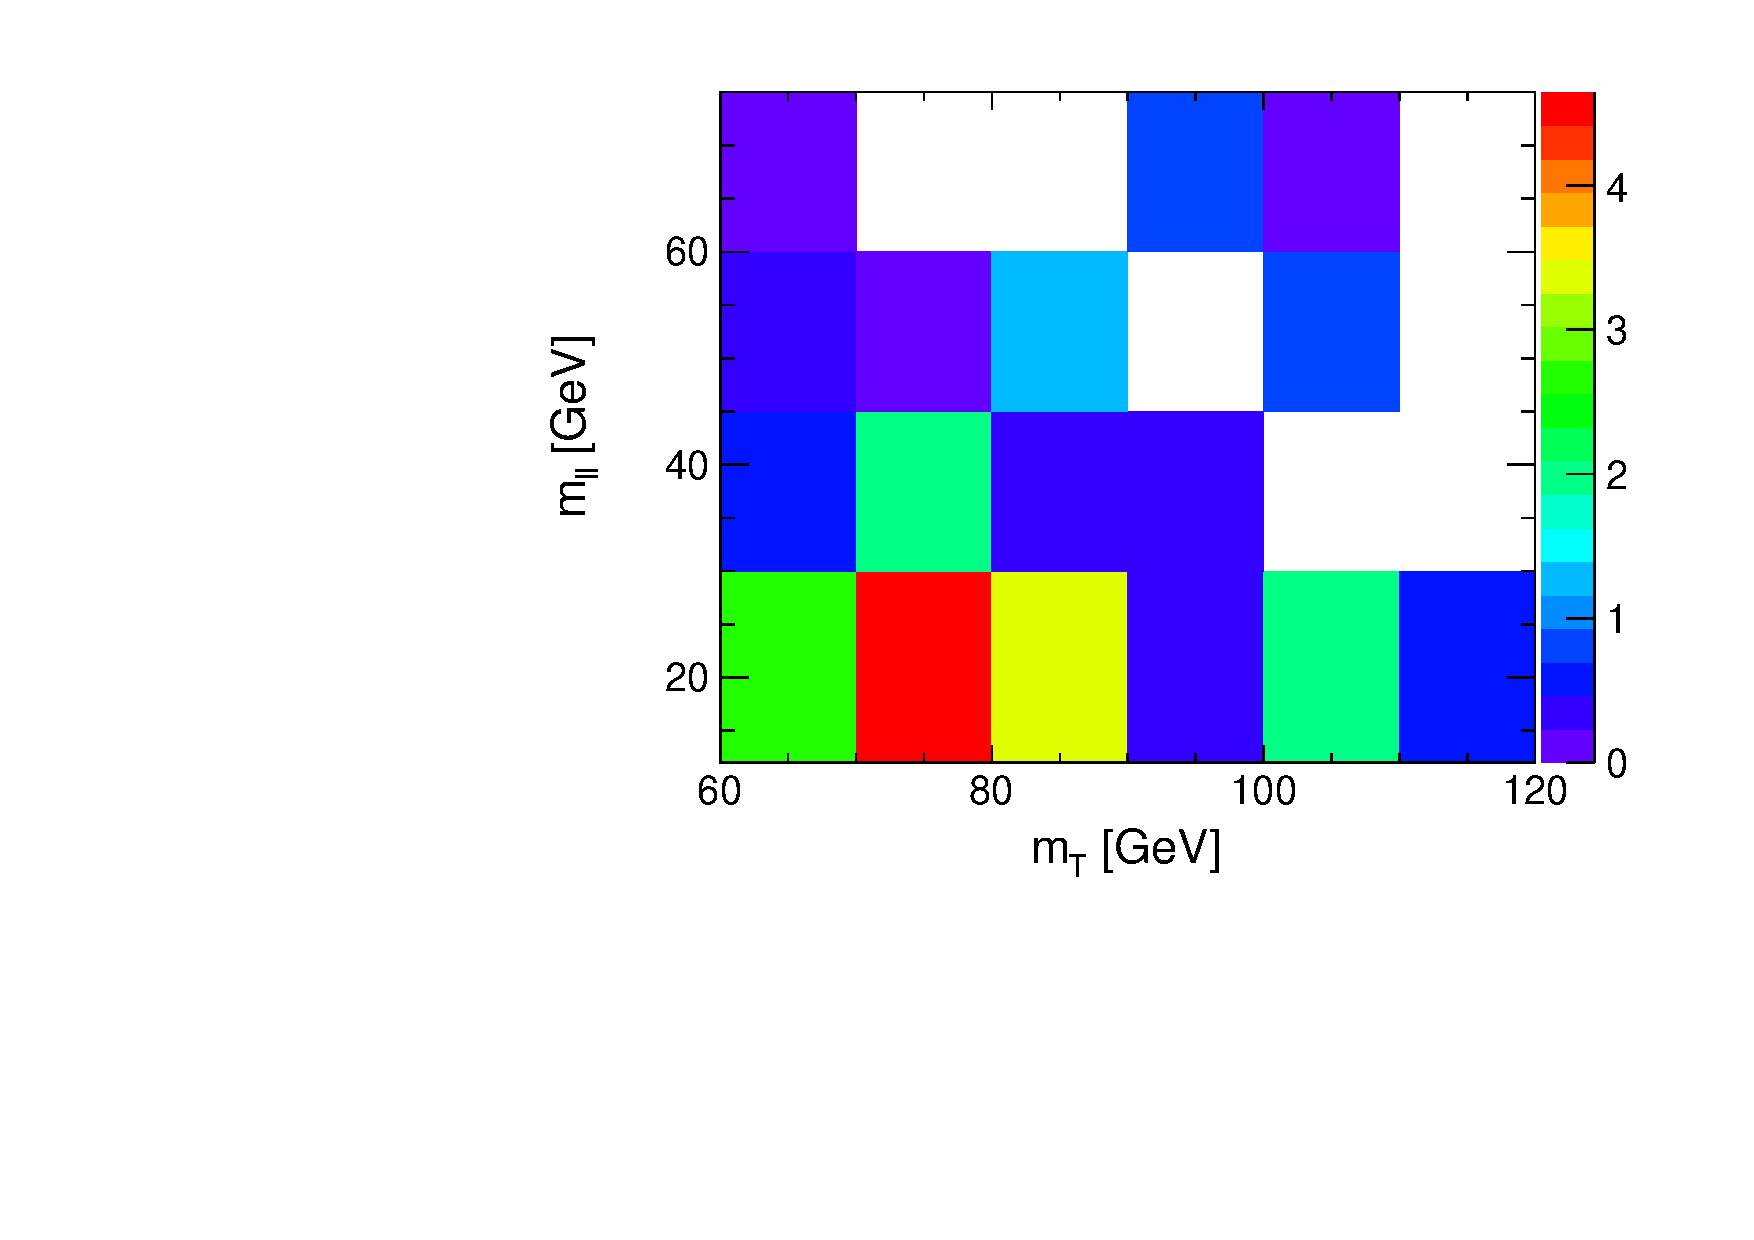
\includegraphics[width=.45\textwidth]{figures/mtvsmll_Wgstar_1j.pdf}
}\\
\caption{The $m_T-m_{\ell\ell}$ templates for the backgrounds, zoomed in 
the signal regions in the {\bf 1-Jet} bin. The distributions are 
normalized to the expectations for \intlumiEightTeV.}
\label{fig:mtvsmll_bkg_1j}
\end{figure}
%%%%%%%%%%%%%%%%%%%%%%%%%%%%%%%%%%%%%%%%%%%%%


\begin{table}[!hbtp]
{%\footnotesize
 %\tiny
 \begin{center}

 \begin{tabular}{|c | c | c c c c c c  }
 \hline
Njet & ggH & qqWW & ggWW & VV & Top & Wjets(E) & Wjets(M) \\ \hline
0    & $237.4\pm49.3$ & $3930.1$ & $208.6\pm62.6$ & $135.7\pm9.7$ & $488.9\pm95.3$  & $275.7\pm99.3$ & $511.8\pm184.2$\\
1    & $91.2\pm28.7$  & $1177.5$ & $67.6\pm 20.3$ & $118.6\pm8.5$ & $1429.4\pm45.7$ & $127.9\pm46.0$ & $226.8\pm81.7$ \\
\hline
\end{tabular}

\vspace{10pt}

 \begin{tabular}{  c c c | c |}
 \hline
  Wgamma & Wg3l & Ztt & $\sum$Bkg \\ \hline
 $123.7\pm37.8$ & $190.8\pm58.4$ & $42.3\pm4.6$ & $5907.6\pm248.5$ \\ 
 $30.7\pm9.4$   & $28.8\pm8.8$   & $73.0\pm8.0$ & $3280.3\pm107.7$ \\
\hline
\end{tabular}
\end{center}
}
\caption{Expected signal and background yields for \intlumiEightTeV. Note that the 
yields of the qqWW process is floated freely in the fits. }
\label{tab:yield}
\end{table}
